% !TEX root = ../my-thesis.tex
%
\chapter{Place du rehaussement dans l'analyse d'images}
\label{sec:SOTA}
Dans ce chapitre, nous présentons les différents filtres de rehaussement de vaisseaux proposés dans la littérature. Afin de remettre dans le bon contexte les problématiques abordées par ces filtres, il est nécessaire de décrire les chaînes de traitement pour l'extraction de vaisseaux sanguins. Pour ce faire, nous introduisons les objectifs de cette extraction sous l'angle de la visualisation des vaisseaux. Nous décrivons ensuite les grandes familles de méthodes de segmentation entrant dans la composition de ces chaînes de traitement.

Dans un second temps, nous montrons l'intérêt des filtres de rehaussement de vaisseaux avant de décrire la manière de les modéliser. Nous démarrons cette présentation en posant les hypothèses sur l'apparence des vaisseaux dans les images. Nous présentons ensuite deux familles distinctes de filtres : les filtres à base de descripteurs matriciels de géométrie et les filtres à descripteurs morphologiques. Dans chacun des cas, nous présentons les espaces d'échelles permettant de capturer les vaisseaux d'une taille donnée, les descripteurs de géométrie associés à l'espace d'échelles et enfin les mesures de tubularité applicables.
\section{Problématiques de la visualisation}
    \newV{Nous avons abordé dans le chapitre précédent les deux méthodes d'acquisition utilisées par l'imagerie du foie en exposant leurs avantages et leurs limites. Nous avons aussi présenté les différentes bases de données publiques disponibles et discuté de leur potentiel en tant que bases d'évaluation d'algorithmes.}

    Bien que nous ayons montré de nombreuses illustrations dans le chapitre précédent, nous n'avons pas abordé la manière de visualiser ces données.
    Le problème initial des médecins est en effet de détecter visuellement des anomalies liées à des pathologies dans ces images. Après les étapes d'acquisition et de reconstruction, les images sont présentées selon deux formes similaires : un ensemble d'images 2D correspondant aux coupes axiales ou un volume 3D, d'un seul bloc, contenant la superposition des coupes.
    
    \newV{La méthode classique d'analyse utilisée par les médecins} est la visualisation des coupes 2D des organes (Fig. \ref{fig:slice_visualization}). De la même manière que la TDM ou l'IRM, le médecin visualise l'image coupe par coupe. Cette visualisation nécessite cependant de l'entrainement et une réelle connaissance des organes étudiés, car le médecin doit reconstituer mentalement le volume des structures observées à partir des images 2D. Cette méthode a toutefois l'avantage de ne nécessiter presque aucun traitement (à part un ajustement dynamique des contrastes) et permet de visualiser l'ensemble de l'image sans problèmes de recouvrement ou d'obstruction entre les structures. 
    \begin{figure}[!ht]
      \centering
      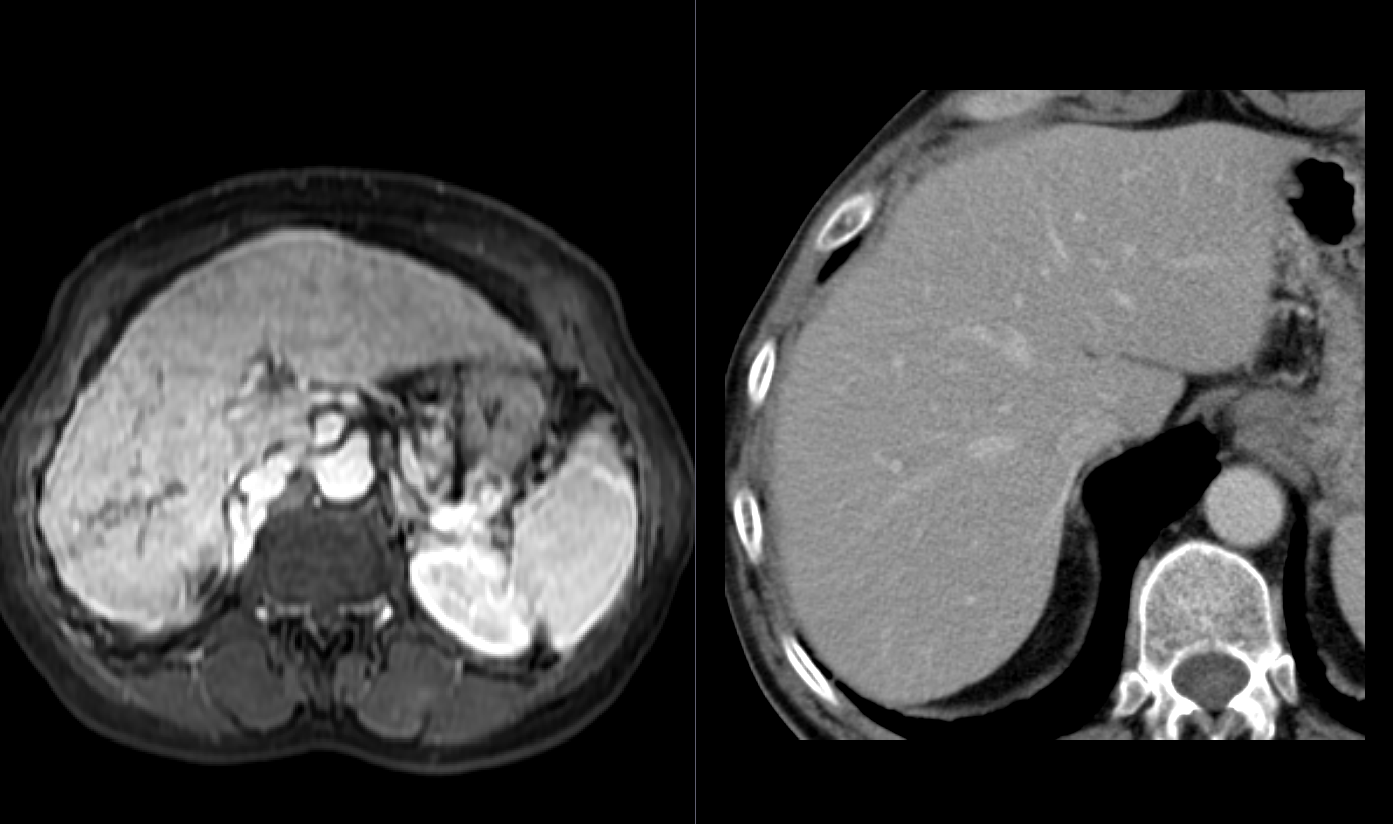
\includegraphics[height=5cm]{Images/2D_view.png}
      \caption{La visualisation en coupes est la méthode la plus utilisée par les médecins. Celle-ci nécessite toutefois de se représenter mentalement la structure 3D de l'organe. À gauche IRM, à droite tomodensitométrie.}
      \label{fig:slice_visualization}
    \end{figure}
    \newV{La visualisation 3D, où l'on travaille avec le volume 3D, facilite cet exercice. Elle permet en effet de visualiser directement les structures dans leur entièreté. Cependant, elle nécessite d'une manière ou d'une autre de hiérarchiser l'information brute de l'image.} Dans le cas contraire, l'information nécessaire au diagnostic reste cachée (Fig. \ref{fig:hierachy_3D}). On peut distinguer deux méthodes pour résoudre ce problème : la première consiste à hiérarchiser les données par projection alors que la seconde identifie et extrait les structures d'intérêt.
    \begin{figure}[!ht]
      \centering
      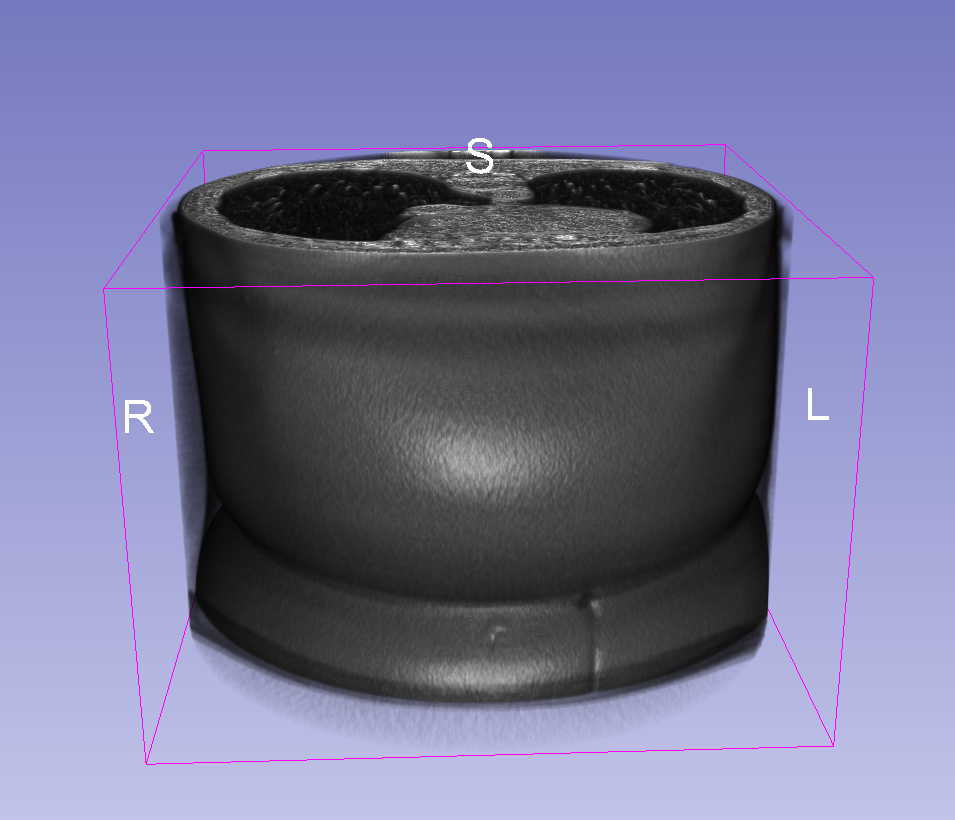
\includegraphics[height=5cm]{Images/hierarchy_3D.png}
      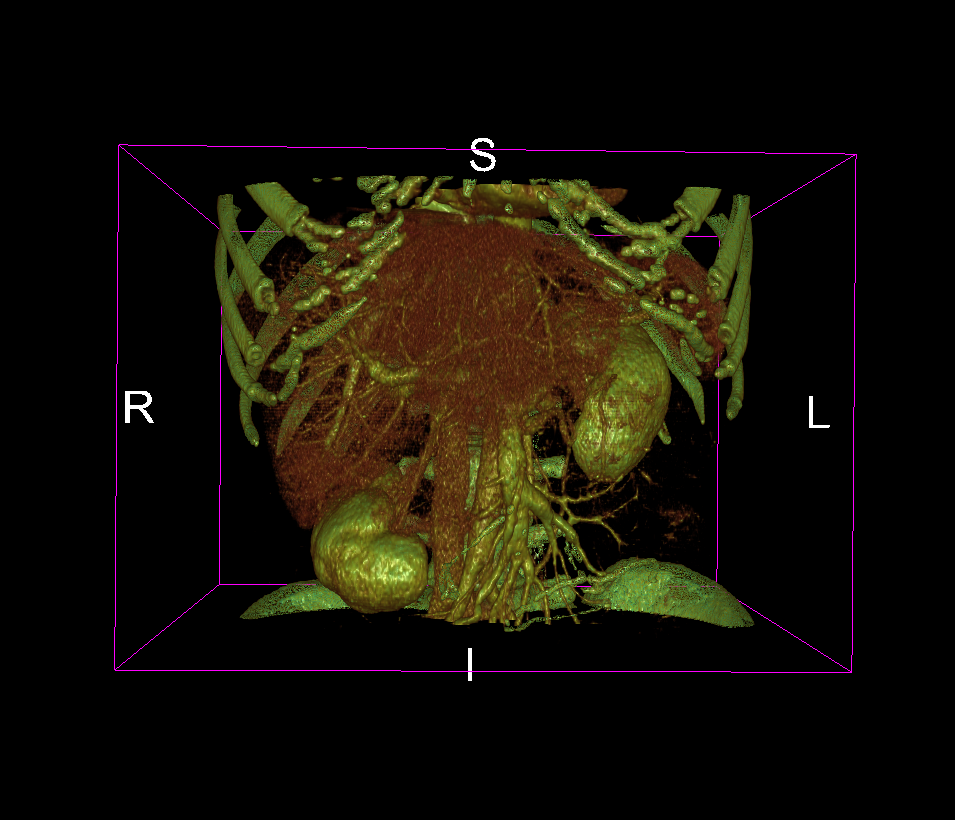
\includegraphics[height=5cm]{Images/hierarchy_3D_bis.png}
      \caption{Rendu surfacique d'un volume 3D. Sans hiérarchisation de l'information, les structures d'intérêt restent cachées. En hiérarchisant l'information (ici un seuil d'opacité et de couleurs en fonction de l'intensité des voxels), on peut observer les structures anatomiques d'intérêt. Un traitement naïf ne suffit toutefois pas à différencier toutes les structures.}
      \label{fig:hierachy_3D}
    \end{figure}
      \subsection{Visualisation par projection}
      La MIP (\textit{Maximum Intensity Projection}) est une technique de projection permettant de visualiser les éléments les plus saillants d'une image. \newV{En pratique, elle consiste à créer un plan image 2D $P$ puis pour chaque pixel $p_i$ de ce plan à lancer un rayon qui traverse le volume 3D. Pour l'ensemble des voxels qui intersectent le rayon, on récupère la valeur maximale parmi leur intensité que l'on affecte à $p_i$ (Fig. \ref{fig:MIP_visualisation}).} 
      \begin{figure}[!ht]
        \centering
        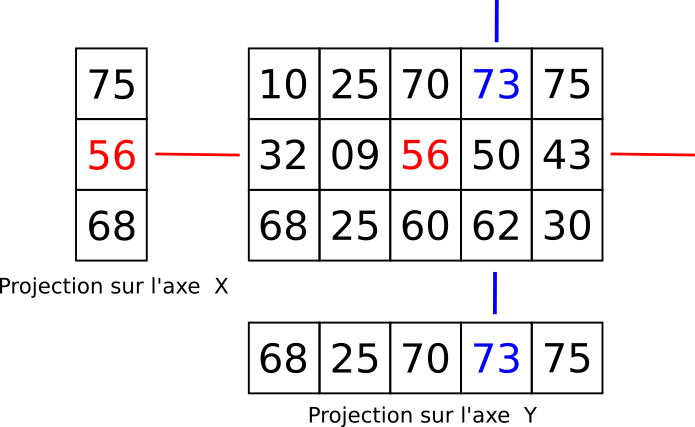
\includegraphics[height=6cm]{Images/3D_mip_ray.png}
        \adjincludegraphics[height=6cm,trim={{0.15\width} {0\height} {0.15\width} {0.15\height}},clip]{Images/3D_mip.png}
        \caption{Maximally intensity projection. L'intensité maximale est projetée le long d'un rayon sur le plan d'origine. La MIP peut s'effectuer en utilisant les axes de l'image ou le plan de la caméra dans une scène 3D.}
        \label{fig:MIP_visualisation}
      \end{figure}
      Cette méthode permet de faire ressortir les éléments les plus intenses de l'image et convient particulièrement à des structures mises en valeur par agent de contraste. Elle est simple à implémenter et peu coûteuse en calcul. Elle fait cependant perdre toute perception de profondeur par la projection des maxima sur le plan image. \newV{On obtient par exemple la même MIP si l'on place le plan de projection avant l'image ou après celle-ci le long de l'axe de projection (à effet miroir près)}.

      La perte de profondeur se compense lorsque dans une scène 3D, le plan de projection devient le plan de la caméra. Le mouvement de la caméra permet alors de résoudre les ambiguïtés provoquées par un seul plan de projection en simulant, dans une certaine mesure, la stéréoscopie de la vision humaine.
      La MIP a aussi le désavantage d'être parasitée par toute structure plus intense que l'organe observé. L'observation du foie et de ses vaisseaux en MIP est notamment perturbée par les os de la cage thoracique. Ce problème peut cependant être contourné en appliquant un masque pour ne conserver que le foie, ce qui demande un coût supplémentaire d'annotation.
      \subsection{Visualisation par isolement des organes}
      D'autres moyens de visualisation sont possibles, par exemple en représentant un modèle 3D des structures observées. On peut ainsi visualiser des organes seuls, sans éléments adjacents perturbateurs (Fig. \ref{fig:segmentation_3D}). La création de ce modèle nécessite un traitement plus complexe des données afin d'identifier, de classer, de filtrer puis d'extraire les structures d'intérêt. C'est cette dernière opération d'extraction que l'on nomme segmentation. La segmentation automatique reste un domaine de recherche ouvert, car les nombreux artefacts de la TDM et de l'IRM complexifient fortement la problématique.
      
      Là où l'utilisation de la MIP est limitée dans ses usages, la segmentation est utilisée non seulement pour la visualisation, mais aussi pour des applications plus larges. Par exemple, elle est nécessaire pour la simulation ou pour le calcul du volume d'un réseau vasculaire, qui sont des tâches pour lesquelles une plus grande précision est demandée.
      
      Dans la suite de ce chapitre, nous présentons les grandes familles d'algorithmes de segmentation avant d'introduire les filtres de rehaussement de vaisseaux qui sont au cœur de nos travaux.
      \begin{figure}[h]
        \centering
        \adjincludegraphics[height=7cm,trim={{0.02\width} {0\height} {0\width} {0.10\height}},clip]{Images/segmentation_3D.png}
        \caption{Segmentation du foie (vert) et des deux réseaux veineux (réseau porte en bleu et réseau hépatique en rose).}
        \label{fig:segmentation_3D}
      \end{figure}
  \section{Extraction de structures d'intérêt}
      Parmi la littérature sur l'extraction de structures d'intérêt, deux sujets sont fortement liés : l'amélioration de la qualité des images et les algorithmes de segmentation.
    \subsection{Amélioration du signal}
    Historiquement, le besoin d'améliorer la qualité des images provient des limitations des premières machines d'imagerie. Il était alors nécessaire de développer des méthodes efficaces pour limiter les artefacts tels que le bruit et ainsi faire ressortir les organes d'intérêt. 
    
    De nombreuses méthodes ont cherché à caractériser, estimer puis corriger le bruit. Par exemple, Gudbjartsson et al. \cite{Gudbjartsson1995r_Rician_noise_MRI} ont explicité le caractère ricien du bruit en IRM. Dietrich et al. \cite{Dietrich2007_measurement_MR_noise} ont proposé une validation des approches pour calculer le rapport signal sur bruit (SNR) en fonction des différentes méthodes d'acquisition et de la reconstruction des images IRM. Gravel et al. \cite{Gravel_2004_estimate_noise_medical_img} proposent une méthode capable d'estimer la nature du bruit en fonction de sa variance et de l'intensité de l'image. Enfin, Krissian et al. \cite{Krissian_2009_diffusion_MRI} et Mendrik et al. \cite{Mendrik2009_HDCS} cherchent à lisser le bruit par un mécanisme de diffusion. Les premiers proposent d'estimer automatiquement le bruit grâce à sa variance pour paramétrer le lissage. Les seconds proposent un lissage adaptatif continu permettant de prendre en compte la géométrie locale.    
    
    De nos jours, les progrès techniques et l'amélioration de la précision des machines ont résolu beaucoup de ces problèmes. La recherche de gains de performances se tourne de plus en plus vers de l'apprentissage qui permet d'améliorer à la fois la qualité des images et d'accélérer les traitements existants. C'est par exemple le cas de méthodes à base de deep learning \cite{Higaki2019_deep_MRI_CT_quality} qui permettent d'améliorer la résolution et de corriger le bruit.

    L'amélioration globale du signal a un effet positif sur les structures anatomiques qui présentent une intensité localement plus homogène ainsi que des contours mieux définis. Leur extraction par des algorithmes de segmentation en est donc facilitée.
    \subsection{Segmentation}
      Les algorithmes d'extraction en imagerie médicale sont les mêmes que l'on retrouve pour des images issues de la photographie classique. \newV{La plupart de ces algorithmes vise à trouver un critère de différenciation entre la structure à extraire et le reste de l'image. Ce critère est souvent défini sous la forme d'une énergie à minimiser.}
      \subsubsection{Contours actifs}
      \newV{Les contours actifs, aussi appelés modèles déformables, cherchent à segmenter un objet en déformant un contour initial fermé afin qu'il s'adapte à la forme de l'objet à segmenter.}
      \paragraph{Contours explicites}
      La méthode développée par Kass et al. \cite{kass1988snakes} (aussi appelés \textit{snakes}) est l'une des méthodes de contours actifs les plus populaires. Cette méthode formule l'énergie contrôlant la propagation du contour comme la somme pondérée d'une énergie interne et d'une énergie externe que l'algorithme cherche à minimiser. L'énergie interne est liée à la modélisation de l'objet que l'on cherche à segmenter et contraint l'expansion du contour (par exemple une énergie liée à un modèle géométrique). À l'inverse, l'énergie externe (basée par exemple sur les gradients de l'image) favorise la propagation du contour. La méthode de Kass et al. a ensuite connu de nombreuses variations comme avec Wang et al. \cite{Wang2012_vessel_level_set} qui proposent un modèle minimisant trois énergies : une énergie basée sur la courbure du contour, une énergie basée sur les gradients d'intensité de l'image et une énergie basée sur la correspondance du contour à un modèle cylindrique. Zeng et al. \cite{Zeng2018_liver_hybrid_active_contour_region_growing} utilisent les contours actifs pour segmenter de gros vaisseaux, sans débordement hors des structures. La paramétrisation du contour actif est basée sur l'estimation de l'intensité des vaisseaux fins détectés par un filtre bi-gaussien.

      L'utilisation des contours actifs est particulièrement efficace sur des objets convexes. Lorsque la géométrie des structures est plus complexe ou très allongée comme pour les vaisseaux, la propagation du contour est plus difficile. \newV{La méthode est aussi moins performante lorsque l'aspect des vaisseaux est bruité et fragmenté}. De plus, l'implémentation du suivi des contours est complexe lorsque des changements de topologie ont lieu. C'est le cas, par exemple, de la séparation du contour en deux contours distincts.
      \paragraph{Contours implicites} 
      \newV{Le problème de suivi de la propagation du contour de la méthode précédente peut être contourné par une formulation implicite des contours. On définit alors un contour comme l'intersection de deux surfaces.} La première surface correspond à l'image vue comme une carte de hauteurs et la seconde surface $\phi$ correspond aux critères de partition (Fig. \ref{fig:level_set}). La dynamique d'évolution du contour implicite est gérée par l'élévation de la surface $\phi$ en fonction du temps. 
      \begin{figure}[!ht]
        \centering
        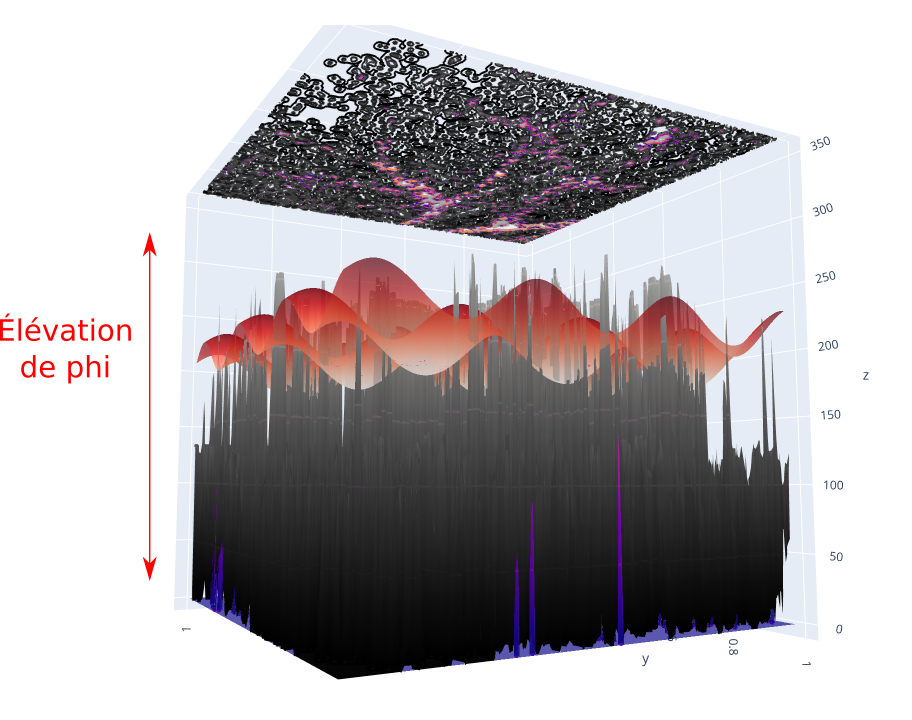
\includegraphics[width=0.45\textwidth]{Images/levelSet_1.png}
        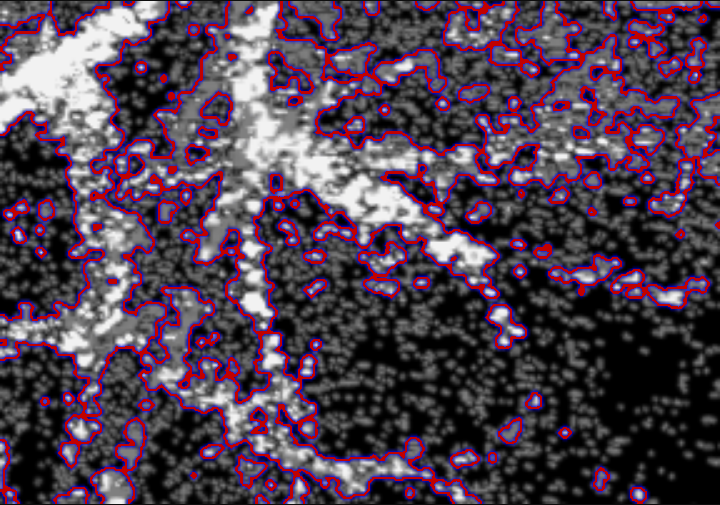
\includegraphics[width=0.45\textwidth]{Images/levelSet_2.png}
        \caption{Illustration des courbes de niveaux. À gauche, les contours sont modélisés comme étant l'intersection de la surface représentant l'image (gris) et d'un critère de partition $\phi$ (surface en rouge). L'évolution du contour est contrôlée par l'élévation de $\phi$. Cette modélisation permet de segmenter le contour de structures déconnectées, visibles sur l'image de droite.}
        \label{fig:level_set}
      \end{figure}
      Li et al. \cite{Li2011_mri_level_set} utilisent les courbes de niveaux pour segmenter des objets malgré une intensité globale non homogène. Pour cela, ils définissent un critère de classification local au voisinage des pixels afin d'estimer un champ de biais d'intensité qui est ensuite incorporé dans l'énergie de propagation.

      \newV{Les contours implicites permettent de segmenter les contours d'objets fragmentés. Cependant, la formulation des courbes de niveaux est généralement plus difficile à définir que pour les contours actifs. Leur mise en œuvre en termes d'implémentation est de ce fait plus complexe.}
      \subsubsection{Graph cut}
      Une image peut aussi être représentée sous la forme d'un graphe. Dans ce graphe, les nœuds sont les pixels et les arêtes encodent une relation de similarité entre ces derniers. Cette relation peut être spatiale où plus complexe. Dans ce contexte, segmenter un objet ou une région revient à trouver la partition qui maximise la vraisemblance à l'intérieur de chaque ensemble et minimise la vraisemblance entre deux ensembles relativement à un critère (Fig. \ref{fig:graph_cut}).
      \begin{figure}[!ht]
        \centering
        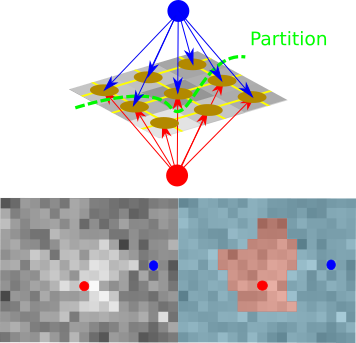
\includegraphics[width=0.5\textwidth]{Images/graph_cut.png}
        \caption{Principe du \textit{graph cut}. Une partition est trouvée en supprimant les arêtes d'un graphe défini à partir des pixels de l'image. Cette partition minimise la vraisemblance entre les deux ensembles, ici des vaisseaux (rouge) et le fond (bleu). }
        \label{fig:graph_cut}
      \end{figure}
      Esneault et al. \cite{Esneault2009_moments_graph_cut} utilisent les graph cuts afin de minimiser une énergie composée de trois critères (région, bordure et vaisseaux). Le modèle de vaisseaux est basé sur un modèle cylindrique. Zeng et al. \cite{Zeng2017_liver_oof_graph_cut} proposent un raffinement d'une segmentation initiale par graph cuts, en utilisant un critère de région basé sur la vraisemblance logarithmique (negative log likelihood) et un critère de bordure basé sur le flux (Sec. \ref{sec:EA:rehaussement:echelle:flux}).
      \subsubsection{Ensemble flou}
      Le choix d'une délimitation entre fond et segmentation n'est pas toujours aisé, en particulier dans les images médicales où les bords des objets à segmenter sont mal définis. La théorie des ensembles flous permet de modéliser cette incertitude. Au lieu d'associer une classe binaire aux pixels, on associe à chaque pixel une probabilité d'appartenance à chaque classe définie pour le problème donné (Fig. \ref{fig:fuzzy_segmentation}). Un critère flou est ensuite construit afin de définir une segmentation binaire définitive.
      \begin{figure}[!ht]
        \centering
        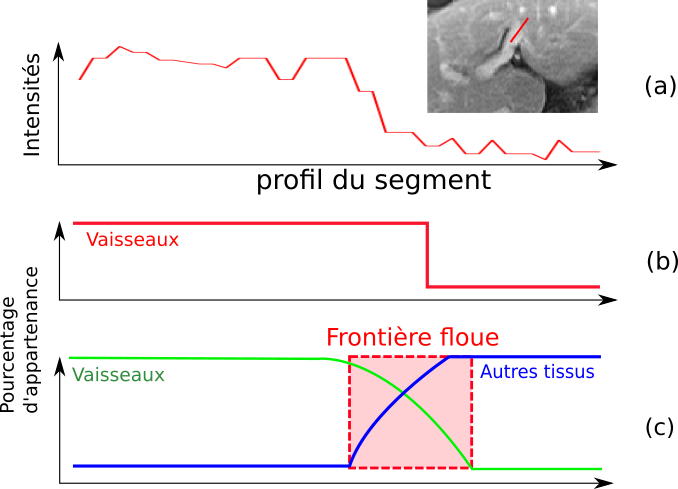
\includegraphics[height=8cm]{Images/fuzzy_segmentation.png}
        \caption{(a) Profil d'intensité des pixels le long du segment. (b) Segmentation binaire : la frontière de la segmentation est nette. (c) Segmentation floue : la frontière de décision est une composition de plusieurs classes qui modélise l'incertitude de la décision.}
        \label{fig:fuzzy_segmentation}
      \end{figure}
      Sigurosson et al. \cite{Sigurosson2014_retinal_morpho_fuzzy} utilisent un ensemble flou pour fusionner l'information provenant de deux ouvertures de chemins pour segmenter les vaisseaux de la rétine. 
      Radojevic et al. \cite{Radojevic2015_fuzzy_logic} détectent les neurones en proposant deux classes floues basées sur le concept de classes multiplicatives. Ils définissent ensuite le degré d'ambiguïté d'un ensemble flou afin d'attribuer une classe finale aux pixels.
      Zhang et al. \cite{Zhang2018_liver_fuzzy_connectedness} définissent un critère de connectivité floue composé d'un critère d'adjacence floue des voxels, et un critère de similarité à la géométrie d'un vaisseau basé sur les filtres de rehaussement de vaisseaux.  
      \subsubsection{Deep learning}
      % Better results with deep learning
      Dans les années 2010, un changement de paradigme a lieu avec l'utilisation croissante des réseaux de neurones. En effet, l'apparition des modèles de réseaux profonds, l'augmentation de la puissance de calculs et un nombre croissant de données annotées ont drastiquement augmenté les performances de ces modèles. Puis, à partir de 2015 les réseaux convolutifs (CNN) prennent une place prépondérante dans la littérature de la segmentation. 
      
      En pratique, on fournit des exemples à un réseau qui produit en réponse une prédiction. L'erreur entre la prédiction et la vérité terrain est ensuite rétro-propagée dans le réseau afin qu'il puisse corriger les prédictions erronées. Ce processus, appliqué de manière itérative sur un grand nombre d'exemples, est appelé entrainement. Deux types d'entraînement sont principalement utilisés, l'entraînement supervisé par paires \{image d'entrée, vérité terrain\} et l'entraînement non supervisé utilisant des images en entrée et une énergie à minimiser qui permet de contraindre la prédiction du réseau.
      % what is used in medical applications
      Dans le domaine médical, ce sont les réseaux convolutifs complets (FCNN), en particulier l'architecture d'auto-encodeur U-Net \cite{Ronneberger2015_Unet}, qui se sont imposés en permettant de segmenter de manière précise des organes. Ce modèle propose une architecture composée d'un encodeur et d'un décodeur symétriques, donnant au réseau sa forme en U caractéristique. Des \textit{skip connections}, permettent de propager les détails de l'encodeur vers le décodeur sans disparaître dans les opérations de rééchantillonages (\textit{pooling}) des couches successives du réseau.

      Plusieurs variantes de ce réseau ont été proposées pour la segmentation des vaisseaux hépatiques, par exemple en combinant Unet et ResNet \cite{yu2019_liver_ResUnet}(Fig. \ref{fig:yu_resunet}) ou DenseNet \cite{Li2018_DenseUnet}. Ces architectures utilisent plusieurs réseaux qui travaillent à des échelles de résolutions différentes ou proposent des branches spécialisées.
      \begin{figure}[!ht]
        \centering
        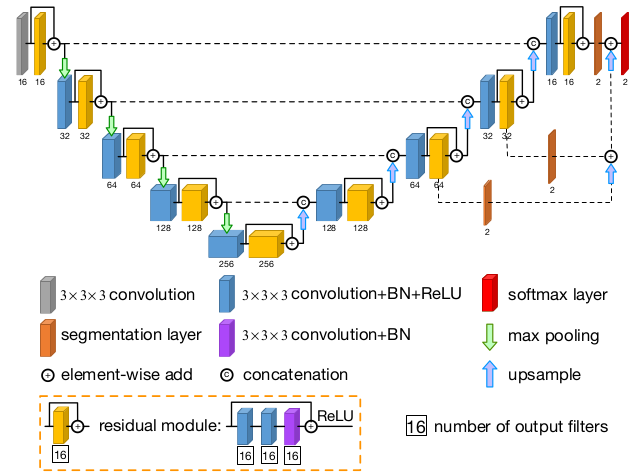
\includegraphics[height=8cm]{Images/Residual_Unet_Yu.png}
        \caption{Architecture \textit{Residual UNet} proposée par Yu et al. \cite{yu2019_liver_ResUnet} pour la segmentation des vaisseaux du foie. Le réseau permet de capturer les structures de plus grandes tailles au fur et à mesure que l'on traverse les couches de l'encodeur en contrepartie d'une perte des détails (partie gauche). Ceux-ci sont ré-incorporés dans le décodeur (partie droite) grâce à des connexions directes (en pointillé). }
        \label{fig:yu_resunet}
      \end{figure}
      Les résultats des réseaux de neurones sont très dépendants de la fonction de coût qui évalue l'erreur entre la prédiction et les données. Pour la segmentation, la \textit{Dice loss} proposées par Sudre \cite{Sudre2017_DiceLoss} s'est popularisée. Cette fonction de coût repose sur le score de Dice qui mesure le recouvrement entre la prédiction et la vérité terrain. Plusieurs métriques similaires ont été proposées et une revue des fonctions de coût pour la segmentation est présentée par Jadon et al. \cite{Jadon2020_survey_seg_loss}. Plus récemment des travaux ont exploré l'introduction de critères topologiques (notamment les composantes connexes) afin de limiter la fragmentation des segmentations ; un problème qui touche les structures fines telles que les vaisseaux \cite{Ventura2017iterative_topo},\cite{Hu2019_topo_homo_persi},\cite{Clough2019_topo_homo_persi}. Ces méthodes restent toutefois très coûteuses en temps de calcul, en particulier lorsqu'elles sont appliquées sur des données 3D. 

      Le nombre des données joue un rôle crucial dans la performance des réseaux de neurones. Cependant, nous avons vu dans le chapitre \chapContextN{} les difficultés de trouver des bases de données publiques avec un nombre important de données bien annotées. 

      Plusieurs méthodes permettent de contourner partiellement ce problème. La plus utilisée est l'augmentation de données \cite{Liskowski2016_data_augmentation}. Celle-ci utilise des données existantes pour appliquer des modifications spatiales ou spectrales des échantillons afin de créer artificiellement des données supplémentaires. D'autres méthodes comptent sur l'utilisation de données partielles, ou d'annotations complètes sur seulement une partie des données \cite{Tajbakhsh2020_imperfect_datasets}. Certains auteurs ont aussi exploré le transfert de style afin de générer des images d'une modalité grâce à des images d'une autre modalité. Chartsias et al. \cite{chartsias2017adversarial} proposent la génération adversaire d'images IRM grâce à des images TDM et un masque d'alignement des structures. Ils montrent qu'en entraînant un réseau à la fois sur des images réelles et générées synthétiquement, on augmente les performances d'un réseau de segmentation. Huo et al. \cite{Huo2018_adversarial} explorent la génération à la fois d'une nouvelle modalité et de sa segmentation.

      Ces méthodes peuvent être intéressantes pour le foie dans la mesure où elles peuvent permettre à un réseau d'apprendre la segmentation des vaisseaux en IRM sans les vérités terrains associées (Fig. \ref{fig:ESSNet}).
      \begin{figure}[!ht]
        \centering
        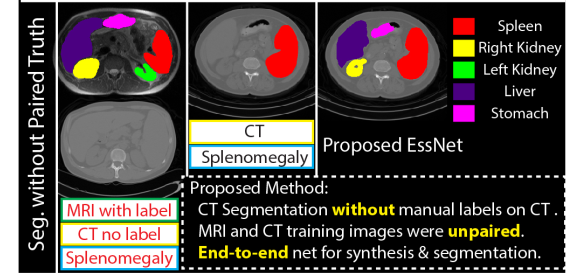
\includegraphics[height=5cm]{Images/ESSNET_application.png}
        \caption{L'apprentissage couplé de la synthèse d'une modalité et de la segmentation associée permet à EssNet (\textit{end-to-end synthesis and segmentation network}) de segmenter une modalité sans annotation manuelle. Travaux de Huo et al. \cite{Huo2018_adversarial}. }
        \label{fig:ESSNet}
      \end{figure}
    \subsection{Problématiques de la segmentation}
    \label{sec:problems_segmenation}
    Créer une chaîne de segmentation est une tâche complexe. Elle doit apporter des réponses efficaces à la fois à la gestion des artefacts d'acquisition des images, de l'apparence des organes à détecter et de l'extraction d'éléments sémantiques de haut niveau. 

    Pour les méthodes sans deep learning, les solutions ont été apportées par l'élaboration de chaînes de traitements complexes. Ainsi, pour la segmentation des vaisseaux hépatiques, Marcan et al. \cite{Marcan2014_vessel_seg} proposent un pipeline de segmentation en 16 étapes mélangeant filtrage du bruit, sélection des éléments pertinents grâce à des masques et analyse des composantes connexes pour la segmentation des vaisseaux du foie. Goceri et al. \cite{Goceri2017_vessel} proposent une méthode en 14 étapes alliant une partition en régions d'intérêt et un étirement du contraste (\textit{contrast stretching}) afin de différencier vaisseaux hépatiques des tissus du foie.
  
    Pour le deep learning, cette complexité se retrouve au niveau de la construction de l'architecture du réseau et de la construction de la base de donnée. Toutefois, si l'on veut effectuer nos traitements en 3D afin de tirer parti de l'ensemble de la géométrie des vaisseaux, les ressources physiques nécessaires deviennent rapidement un goulot d'étranglement.  
    
    Malgré une littérature dense pour la segmentation vasculaire, illustrée dans les revues de Lesage et al. \cite{Lesage2009_review}, Tankyevych et al. \cite{Tankyevych2011_angiographic} et Moccia et al. \cite{Moccia2018_survey} il n'est pas facile de juger de l'efficacité d'une méthode de segmentation par rapport à une autre. Cette difficulté s'illustre dans les tableaux comparatifs de l'état de l'art conduit par  Moccia et al. (Fig. \ref{fig:moccia_table}) qui montrent plusieurs problèmes.
    \begin{figure}[!ht]
      \centering
      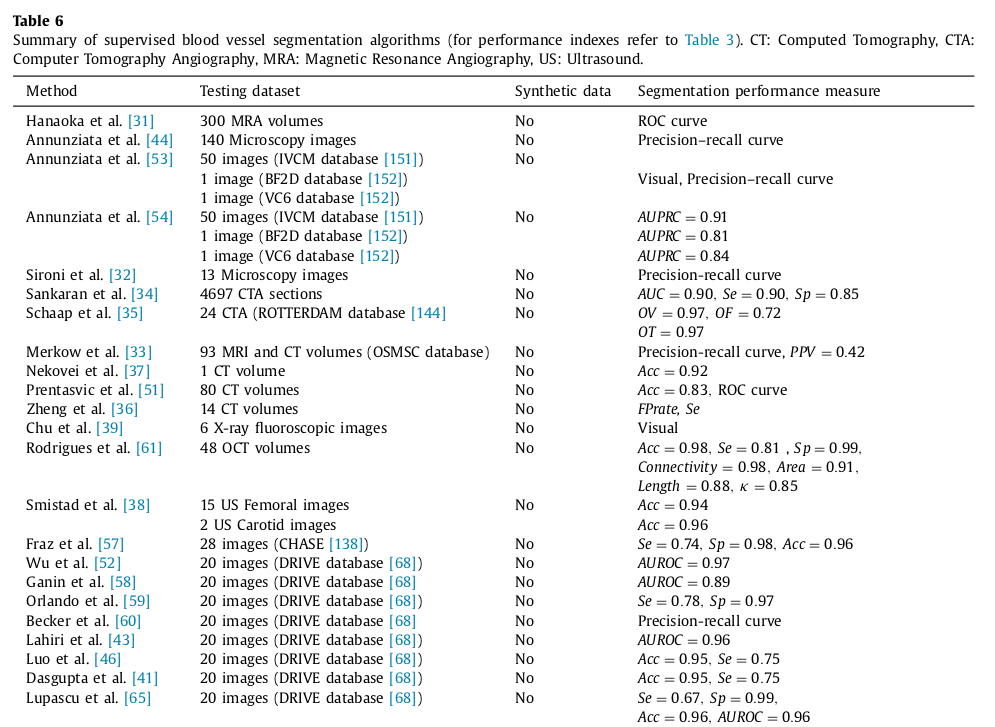
\includegraphics[height=10cm]{Images/Moccia_example.png}
      \caption{Table partielle tirée de Moccia et al. \cite{Moccia2018_survey} récapitulant les résultats de différentes méthodes de segmentation des vaisseaux. Elle illustre la diversité des jeux de données et des méthodes d'évaluations.}
      \label{fig:moccia_table}
    \end{figure}
    Premièrement, il existe une disparité dans les métriques de comparaisons. Certains articles utilisent les métriques standard de classification : précision (\textit{precision}), justesse (\textit{accuracy}), sensibilité, spécificité. D'autres travaux utilisent des métriques de recouvrement comme le Dice ou les coefficients de corrélation de Matthew (MCC) et d'autres des opérateurs intégraux de type \textit{Area Under Curve} (AUC) ou \textit{Receiving Operator} (ROC). Les résultats de certaines méthodes sont mêmes parfois simplement évalués visuellement par des experts.

    Deuxièmement, il y a une hétérogénéité dans les jeux de données. Entre deux articles, il peut y avoir de grandes différences sur le nombre d'images utilisées, les modalités d'acquisition et leur disponibilité. Cette disparité est plus marquée pour les volumes 3D. Des contre-exemples existent comme pour l'imagerie du fond de l'œil (fundus) qui disposent de trois jeux de données annotés qui font référence (DRIVE, STARE, CHASE). L'accessibilité de ces jeux de données annotés est en partie responsable du grand nombre d'articles les utilisant.

    Troisièmement, il est difficile de juger les bénéfices de chaque bloc algorithmique dans une chaîne de segmentation. Une étude ablative, comme on le ferait sur les réseaux de neurones, dans laquelle chaque bloc est retiré afin d'étudier sa performance n'est pas forcément possible. Il est donc complexe de juger si les gains obtenus par une méthode sont atteints grâce à sa modélisation du problème, l'utilisation de caractéristiques particulièrement pertinentes, de la métrique permettant une segmentation efficace ou simplement de la paramétrisation judicieuse de l'algorithme.

    En étudiant plus en détail les blocs algorithmiques utilisés pour la segmentation vasculaire traditionnelle, une famille de filtres est utilisée régulièrement en amont des chaînes de traitement. Leur positionnement en fait un élément clé qui conditionne la suite de la segmentation. Ces filtres ont aussi la possibilité d'être appliqués sur les données d'entrée pour le deep learning. Une étude de leurs propriétés nous paraissait donc pertinente comme un premier pas vers la construction d'un algorithme de segmentation.
\section{Modélisation des filtres de rehaussement}
  \begin{figure}[!ht]
    \centering
    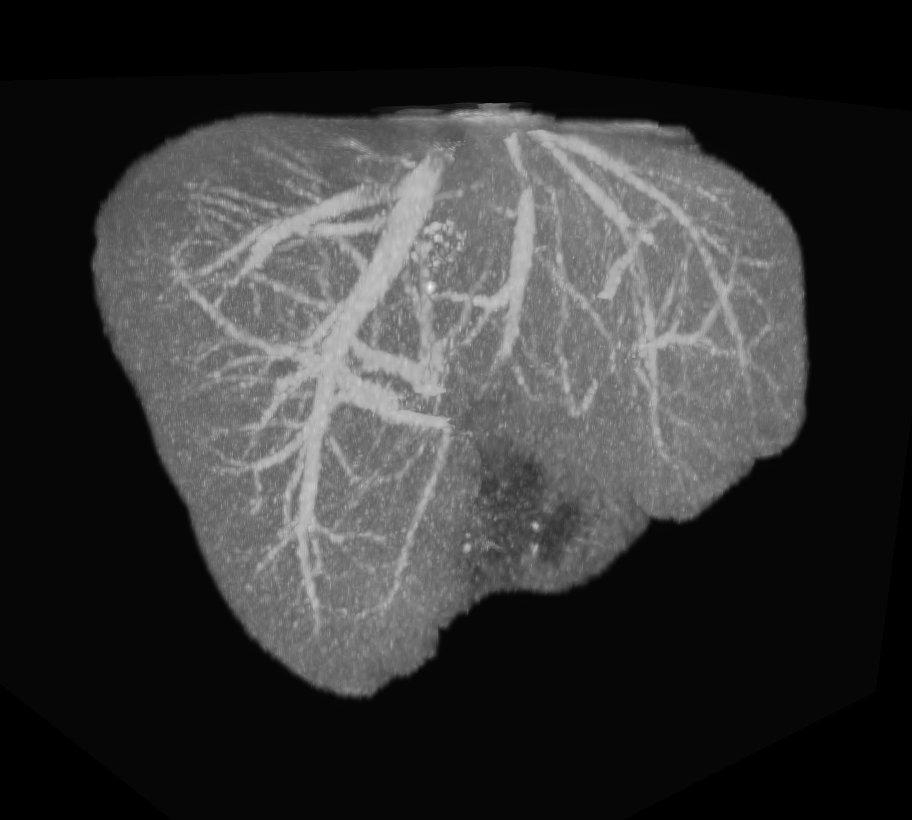
\includegraphics[height=5cm]{Images/enhancement_part1.png}
    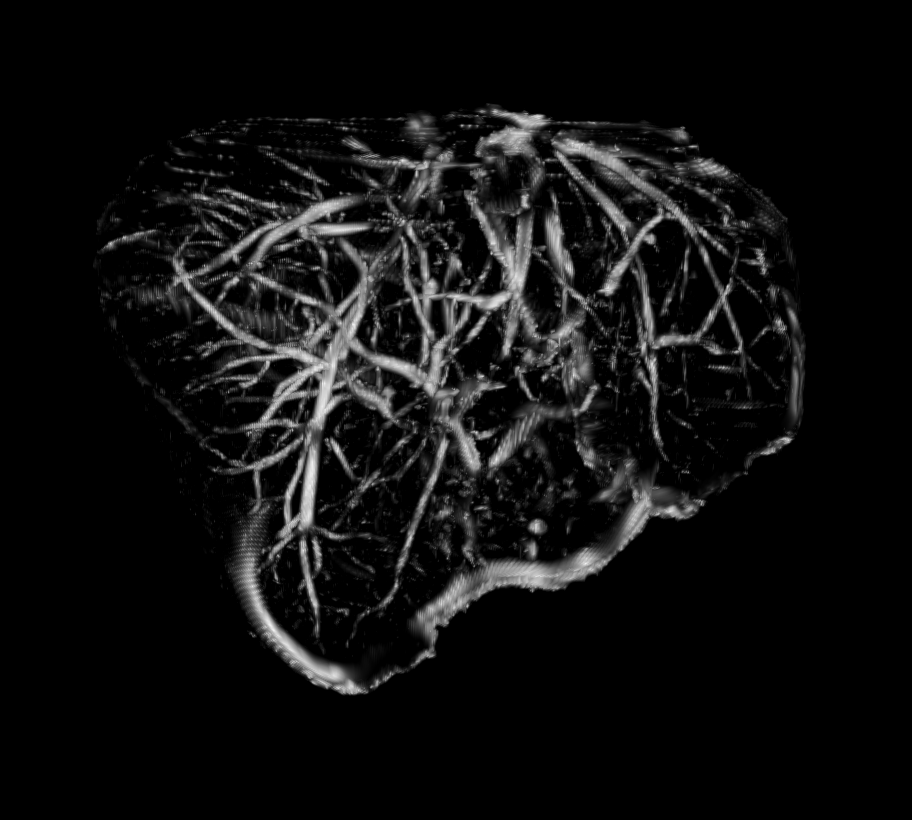
\includegraphics[height=5cm]{Images/enhancement_part2.png}
    \caption{Exemple de filtre de rehaussement de vaisseaux. À droite, un foie en MIP, à gauche les vaisseaux rehaussés. La plupart des vaisseaux inclus dans l'intervalle d'échelles sélectionné sont conservés. Des artefacts de bruit et de bords sont observables.}
    \label{fig:exemple_vesselness}
  \end{figure}
  Les filtres de rehaussement de vaisseaux cherchent à isoler et améliorer le signal des structures géométriques associées à des vaisseaux (Fig. \ref{fig:exemple_vesselness}). Ces filtres répondent pour tout ou partie aux objectifs suivants :
  \begin{itemize}
  \item détecter les structures vasculaires ;
  \item différencier les structures vasculaires des autres structures ;
  \item filtrer les autres structures afin de ne garder que les vaisseaux ;
  \item améliorer le signal des vaisseaux.
  \end{itemize}
Les filtres de rehaussement de vaisseaux reposent sur quatre principes : une modélisation des vaisseaux, un espace d'échelles, un descripteur de structure et une mesure de similarité entre le modèle des vaisseaux et la géométrie mesurée. Ces quatre principes reposent sur des observations effectuées directement à partir des images.
\paragraph{Modélisation des vaisseaux}
\newV{On observe que les vaisseaux sont de longues structures pleines et tortueuses dont la géométrie varie en taille et en courbure. C'est pourquoi la modélisation la plus populaire est d'assimiler les vaisseaux à des structures tubulaires. Les réseaux vasculaires sont formés par la connexion de structures tubulaires qui produisent alors un embranchement. On parle de  bifurcations lorsqu'un vaisseau principal se divise en deux branches, trifurcations en trois et N-furcations dans le cas général. Dans la suite de ce manuscrit, nous effectuons un abus de langage en nommant "bifurcations" l'ensemble des furcations, puisque c'est le cas le plus couramment rencontré. Des hypothèses sont aussi faites sur l'intensité des vaisseaux. Selon les modalités, les vaisseaux peuvent apparaître noirs sur fond plus clair (IRM en phase T1, angiogramme) ou blancs sur fond plus foncé (IRM en phase T2, injection d'agent de contraste). Les hypothèses sont interchangeables, car on peut tout à fait inverser les niveaux de gris de l'image pour passer d'une hypothèse à l'autre. Pour la suite, nous prenons l'hypothèse que les vaisseaux sont clairs sur fond plus sombre.}
\paragraph{Espace d'échelles} 
\newV{Dans un réseau vasculaire, les plus gros vaisseaux peuvent faire plusieurs dizaines de voxels de diamètre tandis que les vaisseaux observables les plus fins peuvent atteindre les limites de la résolution des capteurs et  mesurer jusqu'à un voxel de diamètre. La détection d'un réseau vasculaire dans sa totalité implique de détecter des vaisseaux de différentes tailles. Il n'est cependant pas envisageable de réécrire un algorithme pour chaque taille de vaisseaux ; c'est pourquoi des cadres théoriques, appelés \emph{espaces d'échelles} ont été formulés. Ces espaces d'échelles permettent d'établir un cadre uniforme pour sélectionner les structures d'une image à une échelle donnée. Trois espaces d'échelles sont couramment associés au rehaussement vasculaire dans la littérature : l'espace d'échelles gaussien, l'espace d'échelles de flux orienté et l'espace d'échelles granulométrique.}
\paragraph{Descripteurs de géométrie}
\newV{Mesurer la similarité entre un modèle tubulaire théorique et une structure de l'image nécessite l'utilisation de descripteurs de géométrie. Ces descripteurs sont une représentation compacte, mesurable et locale des caractéristiques d'une structure. Le gradient (le taux de changement d'intensité), la courbure ou la saillance (capacité de la structure à se démarquer du fond) sont des exemples de caractéristiques. Dans la suite de ce chapitre, nous présentons les descripteurs dérivatifs, de phase et à base de flux orienté. Ces trois types de descripteurs ont la particularité d'être des descripteurs matriciels qui peuvent être représentés de manière compacte. Nous présentons ensuite les éléments structurants tubulaires issus de la morphologie mathématique.}
\paragraph{Mesure de tubularité}
\newV{Les mesures de tubularité permettent de déterminer le degré de tubularité d'un voxel par rapport à son voisinage local. Pour les descripteurs matriciels, nous verrons que cette mesure s'exprime comme une combinaison de valeurs propres. Pour les descripteurs de morphologie mathématique le degré de tubularité est principalement dicté par l'élément structurant. Nous verrons cependant un type d'éléments structurants pour lequel la mesure de tubularité repose sur un vote basé sur leurs orientations.}
\newV{Nous avons décrit les quatre principes sur lesquels reposent les filtres de rehaussement de manière indépendante. En pratique, ils sont tributaires les uns des autres à des degrés variables. Par exemple, les descripteurs dérivatifs utilisés avec un espace gaussien peuvent être remplacés par des descripteurs de phase sans difficulté. Ils ne sont cependant pas compatibles avec un espace d'échelles de flux. La morphologie mathématique propose une approche fondamentalement différente, plus proche du \textit{pattern matching}, dans laquelle l'élément structurant est au cœur de l'espace d'échelles et de la description des structures. Dans la suite de ce chapitre, nous présentons les différents composants des filtres de rehaussement tels que présentés dans la table \ref{tab:recap_filters_components} en commençant par les filtres matriciels puis morphologiques.}
\begin{table}[!ht]
  \centering
  \caption{Composants des filtres de rehaussement et leurs affinités. Certains composants des méthodes matricielles sont interchangeables, mais ils ne sont pas compatibles avec les méthodes à base de morphologie mathématique.}
\label{tab:recap_filters_components}
\begin{tabular}{c|c|c}
    \hline
    \multicolumn{3}{c}{Méthodes matricielles} \\
    \hline
    \tbf{Espace d'échelles} & \tbf{Type de descripteur} & \tbf{Mesure de tubularité} \\
    \hline
    \multirow{2}{*}{Gaussien}   & Dérivation   & \multirow{3}{*}{Combinaisons de valeurs propres}  \\
    \cline{2-2}
                                       & Phase        &                                                   \\ 
    \cline{1-2}
    Flux                     & Flux orienté &                                                   \\   
    \hline 
    \hline
    \multicolumn{3}{c}{Méthode par morphologie mathématique} \\
    \hline
    \tbf{Espace d'échelles} & \tbf{Type de descripteur} & \tbf{Mesure de tubularité} \\
    \hline
    \multirow{2}{*}{Granulométrique}             & \multirow{2}{*}{Élément structurant} & Élément structurant \\
                                                        &                                      & Vote sur les orientations \\
  \hline
\end{tabular}
\end{table}
\subsection{Filtres basés descripteurs matriciels}
\newV{Dans cette section, nous présentons d'abord l'espace d'échelles gaussien puis les descripteurs dérivatifs et de phase qui lui sont associés. Nous présentons ensuite l'espace d'échelles de flux et le descripteur de flux orienté. Nous passons ensuite en revue les différentes mesures de tubularité applicables aux descripteurs matriciels.} 
\subsubsection{Espace d'échelles gaussien}
\label{sec:EA:rehaussement:echelle:gaussien}
La théorie de l'espace d'échelles gaussien a été introduit par Lindeberg et al. \cite{Lindeberg1994_scale}. Dans cette théorie, à l'échelle la plus basse, la totalité des structures sont présentes et les détails les plus fins sont conservés. Au fur et à mesure que l'échelle augmente, les détails sont lissés pour ne laisser que les maxima locaux correspondant aux formes les plus grandes. Ainsi, l'échelle minimale correspond à l'image initiale et l'échelle maximale correspond à une image moyennée uniforme (Fig. \ref{fig:gaussian_smoothing}). Lindeberg a aussi montré que les noyaux gaussiens (Eq. \ref{eq:Gaussienne 3D}) étaient les seuls noyaux permettant de passer d'une échelle fine à une échelle grossière sans provoquer l'apparition de nouvelles structures. Au demeurant, un principe identique a été observé dans le fonctionnement de la vision humaine.
\begin{figure}[!ht]
  \centering
  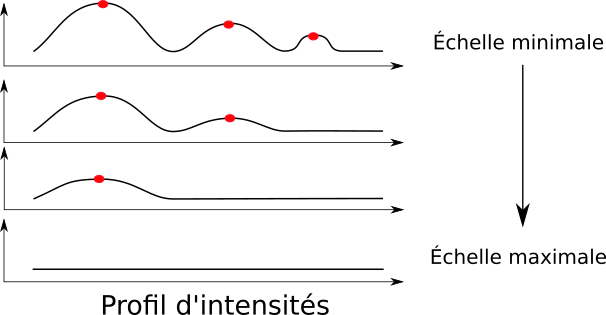
\includegraphics[height=5cm]{Images/gaussian_smoothing.png}
  \caption{Lissage gaussien, les structures de taille égales ou supérieures à $\sigma$ sont conservées. Au fur et à mesure que le lissage augmente, les maxima locaux (rouge) disparaissent progressivement, laissant place à une image uniforme.}
  \label{fig:gaussian_smoothing}
\end{figure}
La sélection de l'échelle dans un espace gaussien se fait par le choix de l'écart-type $\sigma$ de la gaussienne $G_\sigma$ (Fig. \ref{fig:normal_distribution_probability_coverage}, Eq. \ref{eq:Gaussienne 3D}). L'écart-type peut-être défini indépendamment en fonction des axes, mais on considère habituellement un espace d'échelles avec un lissage uniforme dans toutes les directions : $\sigma = \sigma_x = \sigma_y = \sigma_z$. 
\begin{equation}
  G_\sigma(x,y,z) = \frac{1}{ (\sigma\sqrt{2\pi})^3 }\exp(-\frac{x^2 + y^2 + z^2}{2\sigma^2 })
  \label{eq:Gaussienne 3D}
\end{equation}
Il convient de noter que pour un $\sigma$ donné, le diamètre des structures n'est pas supérieur ou égal à $\sigma$, mais plutôt supérieur ou égal à $\alpha\sigma$. En effet, en empruntant le formalisme des statistiques, l'intervalle de confiance, c'est-à-dire la couverture d'une distribution normale, correspond pour $\sigma=1$ à $34.1$ \percent{}, $68$ \percent{}pour $\sigma=2$ et $99.7$ \percent{}pour $\sigma=3$ de la surface de la gaussienne. Ainsi, pour $\sigma=1$ on détectera en théorie des objets de rayon $3\sigma$ et de diamètre $6\sigma$.  
\begin{figure}[!ht]
  \centering
  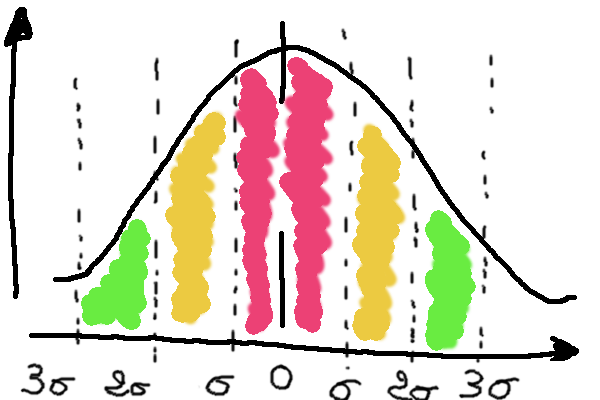
\includegraphics[height=5cm]{Images/normal_distribution_probability_coverage.png}
  \caption{Densité de probablité d'une distribution normale exprimée en pourcentage en fonction de la moyenne $\mu$ et de l'écart type $\sigma$. $99.7$ \percent{}des valeurs sont comprises dans l'intervale $[\mu-3\sigma,\mu+3\sigma]$. Pour un vaisseau, on peut donc prendre hypothèse que la relation entre son diamètre $D$ et la gaussienne de l'espace d'échelles est $D=6\sigma$.\protect\footnotemark}
  \label{fig:normal_distribution_probability_coverage}
\end{figure}

\newV{En pratique l'espace gaussien se calcule par convolution de l'image $I$ avec un noyau gaussien $G_\sigma$ d'écart-type $\sigma$}. Il se prête particulièrement bien à la modélisation des vaisseaux. En effet, la formulation de la gaussienne correspond bien à l'effet combiné des hypothèses de vaisseaux cylindriques et des observations de la diminution d'intensité des vaisseaux au fur et à mesure que l'on s'éloigne de leur centre. Pour un vaisseau de diamètre $3\sigma$, les maxima locaux se situent le long de sa ligne centrale. La justesse de cette hypothèse varie cependant en fonction des modalités et de l'agent de contraste, le flux sanguin étant parfois laminaire et dans d'autres situations turbulent. La gaussienne se prête aussi très bien à une analyse locale de la géométrie basée sur la dérivation. Elle assure en effet les hypothèses de continuité du support de l'image et permet de combiner lissage et dérivation de l'image en une seule étape par dérivation du noyau gaussien. \newV{Les propriétés d'associativité et de commutativité de la convolution rendent possible cette opération :}
\begin{align}
  \frac{\partial}{\partial v} \left[ I(v) \ast G(v) \right] &= \frac{\partial}{\partial v} \ast I(v) \ast G(v) \\
                                                                &= I(v) \ast \frac{\partial}{\partial v} \ast G(v) \\
                                                                &= I(v) \ast \left[ \frac{\partial}{\partial v}G(v) \right]
\end{align}
Enfin, le lissage a l'avantage d'apporter une certaine robustesse au bruit et de compenser la perte locale de signal.\footnotetext{Source : \url{https://en.wikipedia.org/wiki/Normal_distribution}}

L'espace gaussien présente cependant des défauts. Le lissage de l'image implique nécessairement un étalement de toutes les structures qui peuvent par conséquent cacher des formes voisines de plus petite taille. Ce phénomène est particulièrement observé lorsque plusieurs échelles sont étudiées. De même, deux structures adjacentes de même taille peuvent fusionner, et ainsi créer une seule réponse, là où deux objets existaient initialement (Fig. \ref{fig:scale_space_spilling}).
\begin{figure}[!ht]
  \centering
  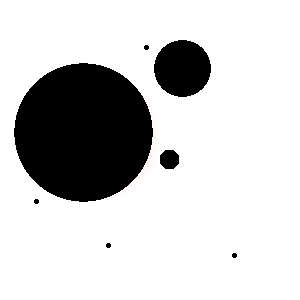
\includegraphics[height=3cm]{Images/gaussian_spilling_init.png}
  
\includegraphics[height=3cm]{Images/gaussian_spilling_g10.png}
  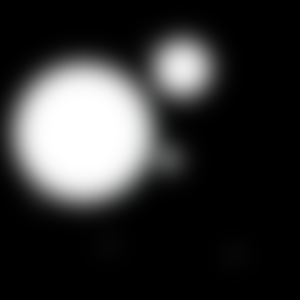
\includegraphics[height=3cm]{Images/gaussian_spilling_g40.png}
  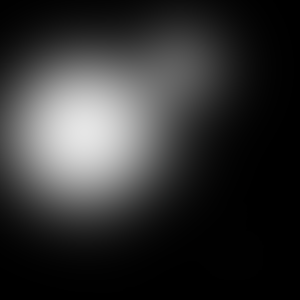
\includegraphics[height=3cm]{Images/gaussian_spilling_g100.png}
  \caption{De gauche à droite, lissage de plus en plus fort par un noyau gaussien. On observe un débordement du signal des structures larges sur les structures de plus petite taille. Ce débordement peut parfois déplacer les maxima locaux vers des points selle.}
  \label{fig:scale_space_spilling}
\end{figure}
\subsubsection{Descripteurs associés à l'espace gaussien}
\subsubsubsection{Descripteurs dérivatifs}
\label{sec:EA:rehaussement:hessienne}
\newV{Les descripteurs dérivatifs permettent de décrire les variations d'intensité autour d'un voxel. Les descripteurs du premier degré décrivent la vitesse de variation des intensités autour d'un voxel. La matrice des dérivées partielles $J$ représentant ces variations dans les trois dimensions est appelée jacobienne (Eq. \ref{eq:jacobian}). Une matrice alternative $S$, le tenseur de structure (Eq. \ref{eq:structure}),  lui est quelquefois substituée \cite{Mendrik2009_HDCS}.}
\begin{equation}
  J(I) =
  \begin{bmatrix}
  j_{1} & j_{2} & j_{3} \\
  j_{1} & j_{2} & j_{3} \\
  j_{1} & j_{2} & j_{3} \\
  \end{bmatrix}
    =
  \begin{bmatrix}
  \frac{\partial I_x}{\partial v_1} & \frac{\partial I_x}{\partial v_2} & \frac{\partial I_x}{\partial v_3} \\
  \frac{\partial I_y}{\partial v_1} & \frac{\partial I_y}{\partial v_2} & \frac{\partial I_y}{\partial v_3} \\
  \frac{\partial I_z}{\partial v_1} & \frac{\partial I_z}{\partial v_2} & \frac{\partial I_z}{\partial v_3} \\
  \end{bmatrix}
  \label{eq:jacobian}
\end{equation}
\begin{equation}
  S(I) =
  \begin{bmatrix}
  s_{1} & s_{2} & s_{3} \\
  s_{1} & s_{2} & s_{3} \\
  s_{1} & s_{2} & s_{3} \\
  \end{bmatrix}
    =
  \begin{bmatrix}
  \left( \frac{\partial I_x}{\partial v_1} \right)^2 & \frac{\partial I_x}{\partial v_2} & \frac{\partial I_x}{\partial v_3} \\
  \frac{\partial I_y}{\partial v_1} & \left( \frac{\partial I_y}{\partial v_2} \right)^2 & \frac{\partial I_y}{\partial v_3} \\
  \frac{\partial I_z}{\partial v_1} & \frac{\partial I_z}{\partial v_2} & \left( \frac{\partial I_z}{\partial v_3} \right)^2 \\
  \end{bmatrix}
  \label{eq:structure}
\end{equation}
Pour les vaisseaux sanguins, qui peuvent être vu comme des maxima locaux étroits, la description de la courbure des intensités autour d'un voxel est plus pertinente. Cette courbure est décrite par la matrice des dérivées partielles secondes $H$ : la matrice hessienne (Eq. \ref{eq:hessian_matrix}). 

Les valeurs propres et les vecteurs propres issus de la hessienne sont une représentation compacte des variations exprimées par la matrice. Les vecteurs propres permettent d'exprimer les directions principales de la courbure (pour la hessienne) et les valeurs propres expriment la force de la courbure pour chaque direction.
Les valeurs propres et vecteurs propres de la hessienne permettent de quantifier l'orientation, le sens et l'amplitude du voisinage d'un point. L'utilisation des valeurs propres est explicité dans la section \ref{sec:mesure_tubularity}.
\begin{equation}
  H(I) =
  \begin{bmatrix}
  h_{11} & h_{12} & h_{13} \\
  h_{21} & h_{22} & h_{23} \\
  h_{31} & h_{32} & h_{33} \\
  \end{bmatrix}
    =
  \begin{bmatrix}
  \frac{\partial^2 I_x}{\partial v^2_1} & \frac{\partial^2 I_x}{\partial v_1 \partial v_2} & \frac{\partial^2 I_x}{\partial v_1 \partial v_3} \\
  \frac{\partial^2 I_y}{\partial v_2 \partial v_1} & \frac{\partial^2 I_y}{\partial v^2_2} & \frac{\partial^2 I_y}{\partial v_2 \partial v_3} \\
  \frac{\partial^2 I_z}{\partial v_3 \partial v_1} & \frac{\partial^2 I_z}{\partial v_3 \partial v_2} & \frac{\partial^2 I_z}{\partial v^2_3} \\
  \end{bmatrix}
  \label{eq:hessian_matrix}
\end{equation}
\subsubsubsection{Descripteurs de phase}
\label{sec:EA:rehaussement:Phase}
Une image peut-être à la fois vue comme une matrice de pixels et comme un signal sinusoïdal discret en 2 ou 3 dimensions. \newV{La représentation sous forme de signal dépend de deux paramètres : l'amplitude, correspondant à l'intensité des pixels, et la phase correspond au décalage temporel ou spatial de ce signal. En pratique on s'intéresse plutôt à la mesure de la différence de phase entre les périodes de deux signaux (Fig. \ref{fig:phase_shift}).}
\begin{figure}[!ht]
  \centering
  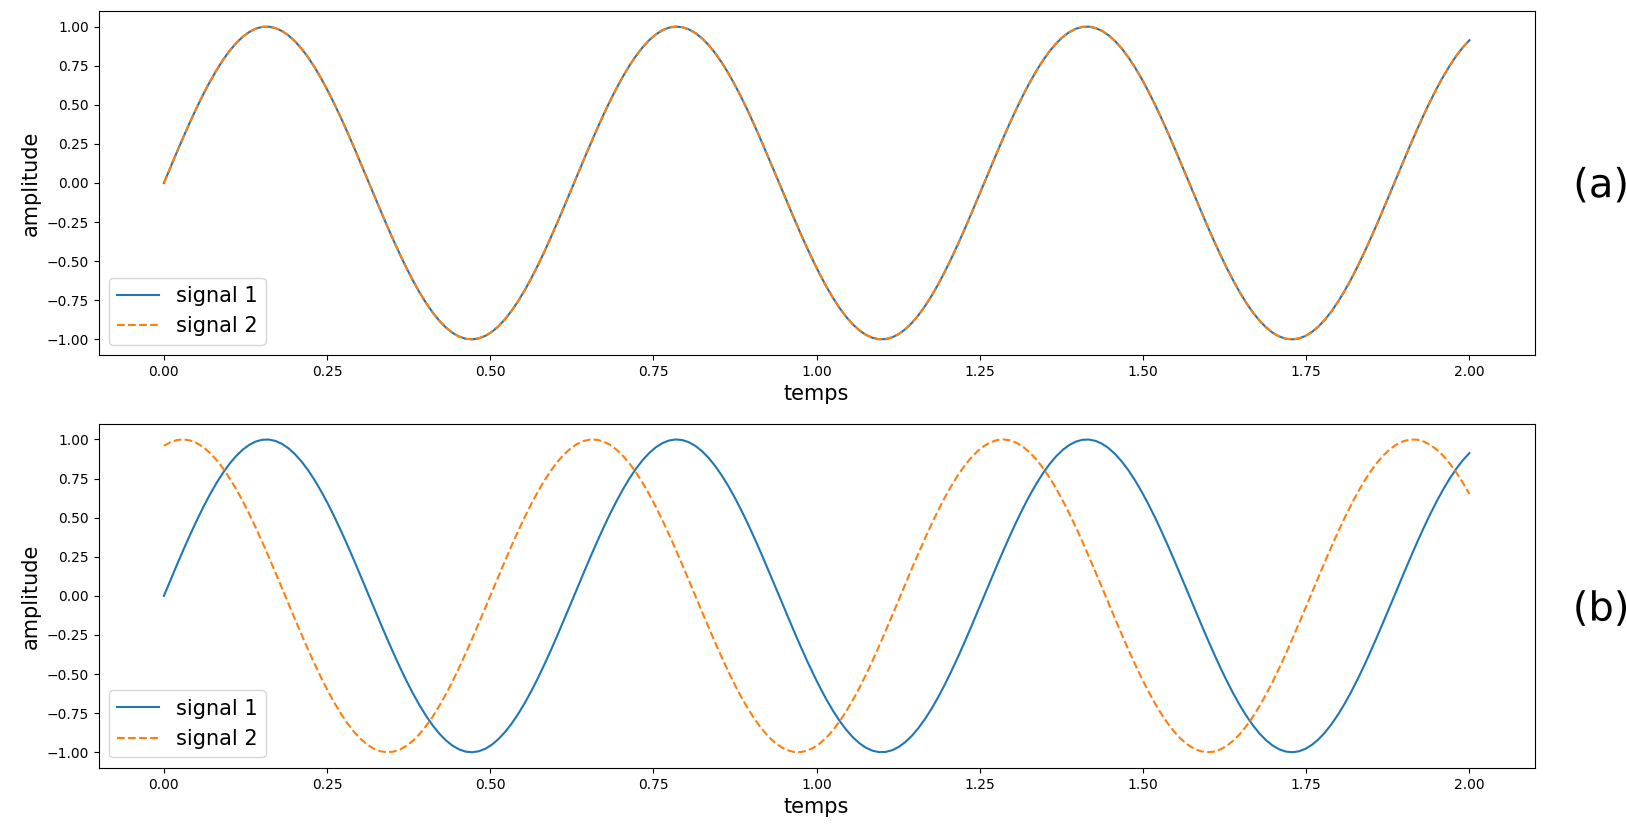
\includegraphics[height=5cm]{Images/phase_shift.png}
  \caption{(a) Signaux à phase et amplitude égale. (b) signaux à amplitude égale avec des phases différentes. La différence de phase mesure le décalage temporel entre les deux signaux.}
  \label{fig:phase_shift}
\end{figure}
La phase est indépendante de l'amplitude et n'est donc pas affectée par des changements d'intensité. Oppenhei et al. \cite{Oppenheim1981_phase_importance} démontrent l'importance de ces caractéristiques de l'image et montrent une correspondance avec le système visuel humain. 
\begin{figure}[!ht]
  \centering
  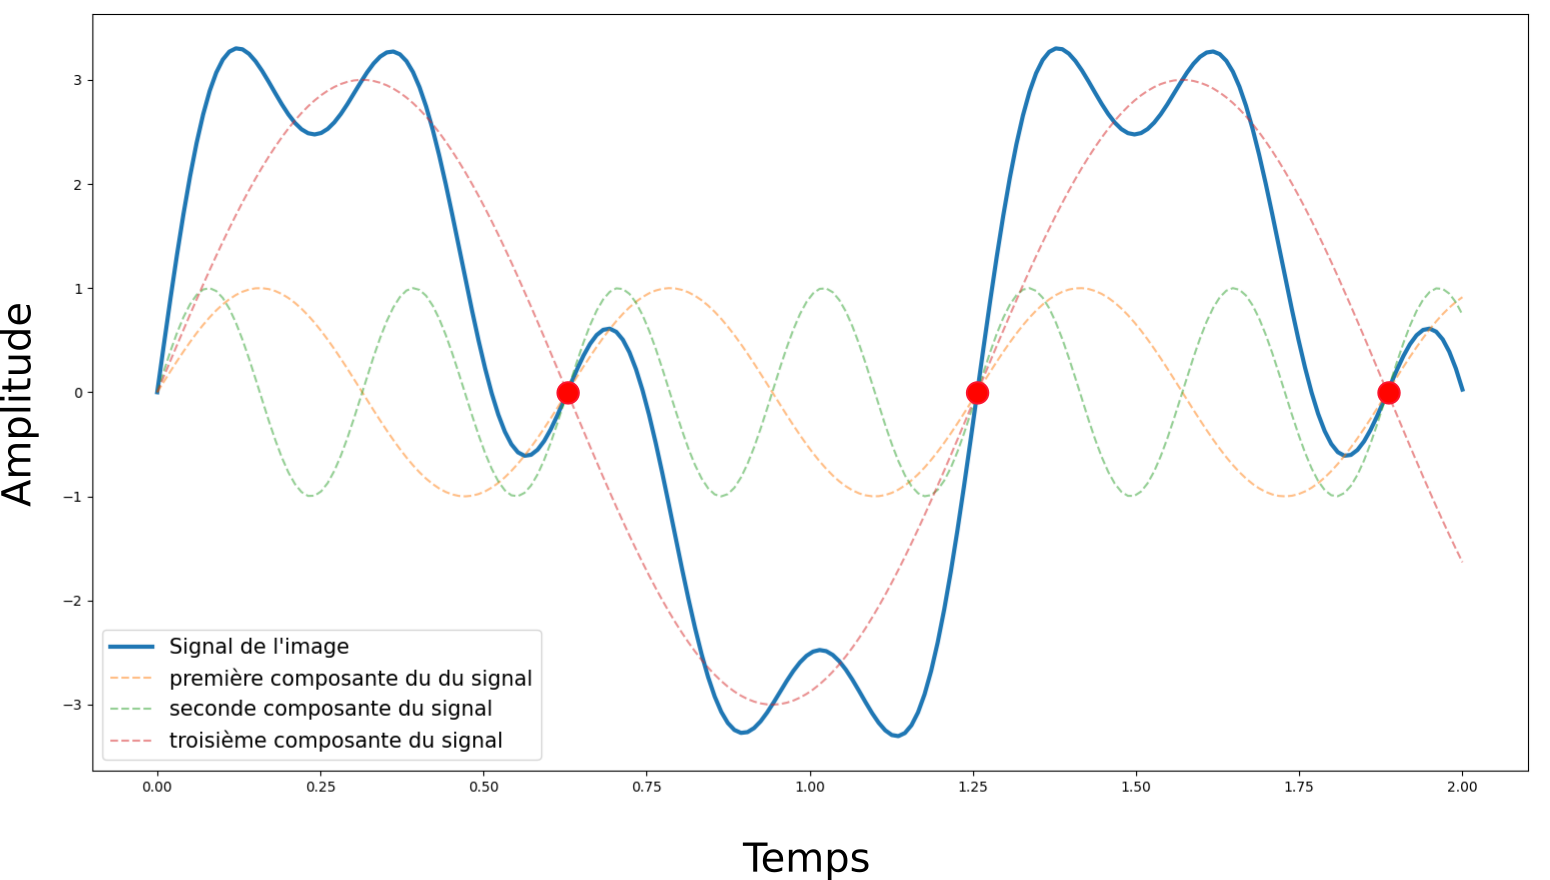
\includegraphics[height=5cm]{Images/PC_decomposition.png}
  \caption{Décomposition de Fourier d'un signal. En certains points (rouge) la phase de chaque composante du signal est synchronisée. Ces points correspondent aux éléments saillants des images et sont indépendants des variations d'intensité (amplitude) de l'image. Le contraste de phase correspond à la mesure de la synchronisation des phases des composantes du signal.}
  \label{fig:phase_congruency}
\end{figure}

Plusieurs constructions de filtres de rehaussement se basent sur cette propriété pour la détection des vaisseaux. Obara et al. \cite{Obara2012_phase} utilisent un tenseur de structure basé sur le contraste de phase (Fig. \ref{fig:phase_congruency}). Les valeurs propres de ce tenseur permettent ensuite d'exprimer une mesure de tubularité.

Ce tenseur est exprimé comme :
\begin{equation}
  T_{PC} = \sum_o PC_{o}(p)(n_{o}n^T - \alpha \text{I})
\end{equation}
avec $PC(x)$ la fonction de congruence de phase, $n_{\theta}=[cos(\theta),sin(\theta)]^T$ le vecteur d'orientation $o$, $I$ le tenseur unitaire, $\alpha = 1/(m-1)$ avec $m$ la dimension de $I$. $PC(x)$ permet de détecter les éléments saillants à la manière d'un détecteur de contours.
En effet, une image vue comme un signal peut être décomposée comme un ensemble de signaux sinusoïdaux. Les éléments saillants tels que les bordures ou les coins d'objets correspondent à une synchronisation, e.g congruence, de ces signaux pour un angle donné. La congruence de phase s'exprime par :
\begin{equation}
  PC(x) = max_{\theta \in [0,2\pi)}  \frac{\sum_\omega \alpha_{\omega}cos(\omega x + \phi_{\omega} - \omega)  }{\sum_\omega \alpha_{\omega} }
\end{equation}
Elle représente la variance de phase des différents signaux au point $x$. Lorsque les phases des signaux sont égales, $PC(x)=1$.
En pratique, cette définition est complexe à implémenter. On lui préfère la mesure d'énergie locale qui s'approxime avec des filtres de Gabor ou des ondelettes. Ces filtres sont basés sur des gaussiennes dont on peut contrôler l'échelle comme un espace gaussien.

Enfin, ces filtres sont dépendants du nombre d'orientations échantillonnées $\omega$. En pratique entre 6 et 10 échantillons régulièrement espacés suffisent en 2D. 
\subsubsection{Espace d'échelles de flux}
  \label{sec:EA:rehaussement:echelle:flux}
  \newV{Comme nous l'avons vu dans la section \ref{sec:EA:rehaussement:echelle:gaussien}, l'espace d'échelles gaussien peut provoquer des débordements de structures sur d'autres, plus petites. On peut limiter ce problème en utilisant un cadre différent, celui de l'analyse des flux.} 
  
  Si l'on considère un champ de vecteur $V$, par exemple un champ de gradient pour une image, on définit le flux (Eq. \ref{eq:flux}) passant à travers une surface $S$, orienté par sa normale $\vec{n_s}$, comme l'intégrale de la somme du produit scalaire entre \newV{le champ de gradient $\vec{v}$} et la normale à la surface $\vec{n}$.
  \begin{equation}
  flux_S = \int_{S}< \vec{v},\vec{n} > dS
  \label{eq:flux}
  \end{equation}
  \newV{Le calcul du flux s'applique à la surface d'un objet fermé dont les frontières sont clairements définies. On évite donc, par construction, le débordement observé avec l'espace gaussien. Les structures en forme de disques, de sphères \cite{Law2008_OOF} ou de cylindres \cite{Wang2019_cylindrical_flux} sont utilisées pour la détection des vaisseaux. Dans ce contexte, l'échelle est définie par la taille de la surface sur laquelle est calculée le flux. Pour un disque et une sphère, le paramètre d'échelle correspond donc au diamètre de l'objet. Cette formulation de l'échelle diffère des méthodes précédentes, car les objets tubulaires ne sont détectés que pour une échelle donnée, là où les deux autres techniques conservent les objets à l'échelle donnée et aux échelles supérieures. Elle a aussi l'avantage de limiter l'analyse du flux à la surface de la sphère et donc de produire une réponse qui ne déborde pas.}

  \newV{Afin de garantir une précision constante du calcul du flux, il est nécessaire d'échantilloner la surface de la sphère à intervalle réguliers et constants peu importe la taille de $S$. Plus l'échelle sélectionnée est grande, et donc plus la surface de la sphère est grande, plus le nombre d'échantillons requis est important. Cette contrainte fait croître le coût en calcul proportionnellement à la taille de la sphère.} Law et al. \cite{Law2009_efficient_implementation} proposent une formulation élégante du calcul de flux dans le domaine de Fourier afin de réduire drastiquement le temps de calcul par rapport à l'implémentation naïve.
  Pour y parvenir, ils proposent d'exprimer le calcul de flux sous la forme d'une convolution dans le domaine temporel. L'avantage de la convolution est double : on évite l'étape d'échantillonnage sur la surface et la convolution s'exprime comme une multiplication dans le domaine de Fourier. On peut exprimer le calcul de flux en termes de volume et non plus en termes de surface grâce au théorème de la divergence qui établit une égalité entre le flux à la surface d'un objet et le flux à l'intérieur de son volume. Ainsi :
  \begin{equation}
    flux_{C} = \int_{\partial C}< \vec{v},\vec{n} > d\rho \equiv \int_{C }\Delta I d\nu
  \end{equation}
  Plus précisément la forme continue du flux $f_s$ est définie par :
  \begin{equation}
    f_s(x,y,z) = \int_{\partial R_s}\vec{v}(x+t,y+p, z+q) . \vec{n}_{(t,p,q)}dA
    \label{eq:next_oof}
  \end{equation}
  avec $R_s$ une région sphérique de rayon $s$, $dA$ une surface infinitésimale sur la surface $\partial R_s$, $\vec{n}_{(t,p,q)}$ le vecteur normal à $dA$ à la position $(t,p,q)$ et $\vec{v}$ le gradient de l'image $I$. $\vec{v}$ est obtenu à partir de l'image $I$ lissée par un noyau gaussien (i.e. $\vec{v}=\nabla(g)*I)$.) afin d'assurer la dérivabilité du signal de $I$ comme explicité dans la section \ref{sec:EA:rehaussement:hessienne}.
  Eq. \ref{eq:next_oof} est équivalente à :
  \begin{align}
    f_s(x,y,z) & = \int_{R_s} \vec{div}( \vec{v}(x+t,y+p, z+q) ) dtdpdq \\
    \nonumber
    & = \int_{\omega} d_s(t,p,q) \vec{div}( \vec{v}(x+t,y+p, z+q) ) dtdpdq
  \end{align}
  où $\omega$ est le domaine entier de l'image et $d_s(t,p,q)$ correspond à la fonction porte sphérique de rayon $s$ définie par :
  \begin{align}
    d_s(x,y,z) & = \begin{cases} 
                  1, \sqrt{x^2 + y^2 + z^2} \leq s  \\
                  0, \text{sinon} \\
                \end{cases}
  \end{align}
  Ainsi, $f_s(x,y,z)$ peut être reformulée sous forme de convolution :
  \begin{align}
    f_s(x,y,z) & = \int_{\omega} d_s(t,p,q) \vec{div}( \vec{v}(x+t,y+p, z+q) ) dtdpdq \\
              \nonumber
               & = \int_{\omega} d_s(t,p,q) (\Delta(g*I(x+t,y+p, z+q))) dtdpdq \\
               \nonumber
               & = \int_{\omega} d_s(-t,-p,-q) (\Delta(g*I(x+t,y+p, z+q))) dtdpdq \\
               \nonumber
               & = I(x,y,z) * d_s * \Delta g \\
               \nonumber
               & = I * h_s(x,y,z)
    \label{eq:oof_next2}
  \end{align}
  avec $*$ l'opérateur de convolution, $\Delta$ l'opérateur laplacien.
  L'équation \ref{eq:oof_next2} exprimée dans le domaine de Fourier donne :
  \begin{align}
    FFT( I * h_s(x,y,z) ) &= FFT(I) . FFT(h_s(u,v,w)) \\
                          \nonumber
                          &= FFT(I) . FFT(ds(u,v,w)) . (j2 \pi)^2 ( (\frac{u}{N_x})^2 + (\frac{v}{N_y})^2 + (\frac{w}{N_z})^2 )  \\
                          \nonumber
                          & . \exp( -( (\frac{u}{N_x})^2 + (\frac{v}{N_y})^2 + (\frac{w}{N_z})^2 ) 2(\pi\sigma)^2 )
  \end{align}
  \newV{avec $N_x$, $N_y$ et $N_z$ les dimensions de l'image le long respectivement des axes $x$, $y$ et $z$.}
\subsubsection{Descripteurs associés à l'espace d'échelles de flux}
\subsubsubsection{Flux orienté sphérique}
 \newV{La structure utilisée pour le calcul de flux orienté sphérique est une sphère $S_r$ de rayon $r$.} Une matrice $Q$ qui décrit la géométrie locale au niveau de la sphère est calculée à partir du champ de gradient sortant de la surface de la sphère $S_r$. Les auteurs formulent ainsi un problème d'optimisation cherchant à trouver une direction de projection optimale  $\widehat{\rho}$ qui minimise le flux entrant dans la sphère. Cette formulation est définie par :
\begin{equation}
    f(x;r, \widehat{\rho} )= \int_{\delta S_r} (( v(x + r\widehat{n}).\widehat{\rho})\widehat{\rho}). \widehat{n}\,dA = \widehat{\rho}^{T}Q_{r,x}\widehat{\rho}  	\nonumber
\end{equation}
où $v(.)$ correspond au gradient de l'image à la position ".", $dA$ est une zone infinitésimale sur la surface $\delta S_r$ et $\widehat{n}$ la normale unitaire orientée vers l'extérieur de la sphère $\delta S_r$.
Les $i^{ème}$ ligne et $j^{ème}$ colonne de $Q$ sont définies par: 
\begin{equation}
    q_{r,x}^{i,j} = \int_{\delta S_r} (( v_i(x + r\widehat{n}).\widehat{\rho})\widehat{\rho}).n_j\,dA = \widehat{\rho}^{T}Q_{r,x}\widehat{\rho}  \nonumber	
\end{equation}
En pratique, le flux entrant est minimal quand le flux sortant est maximisé, c'est-à-dire lorsque la sphère est positionnée au centre d'un vaisseaux. Dans ce cas, l'orientation optimale de projection correspond à la direction de la ligne centrale du vaisseau. Les valeurs propres de la matrice résultante peuvent être exploitées comme celles de la matrice hessienne. Law et al. \cite{Law2008_OOF} définissent d'ailleurs une relation d'équivalence entre $Q$ et la matrice hessienne.
\subsubsection{Mesures de tubularité}
\label{sec:mesure_tubularity}
\newV{Basées sur les espaces d'échelles et les descripteurs matriciels vu précédemment, plusieurs mesures de tubularité ont été proposées dans la littérature. Nous n'évoquerons ici que le cas de la hessienne, puisque nous avons vu que la matrice de flux orienté $Q$ lui était équivalente. Les mesures de tubularité reposent sur une représentation condensée de ces matrices : les vecteurs propres et les valeurs propres.}

\newV{La matrice hessienne telle que nous l'avons formulée est exprimée par rapport aux axes $x$, $y$ et $z$ de l'image. Les vecteurs propres forment une base vectorielle orthogonale différente de la base utilisée dans la matrice hessienne. Les vecteurs propres sont ainsi orientés dans les directions principales des variations de courbure d'intensité du voisinage d'un voxel. Les valeurs propres sont des facteurs d'homothétie des vecteurs propres et correspondent à la force de la variation de courbure des intensités dans le sens du vecteur propre associé (Fig. \ref{fig:ev}).}
\begin{figure}
\centering
  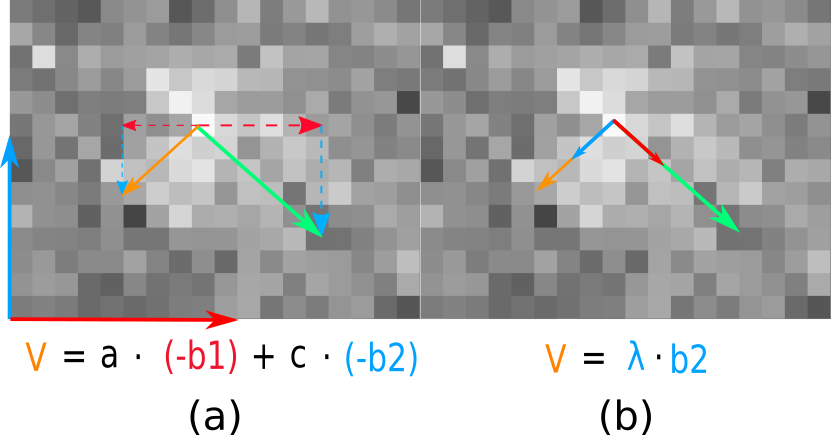
\includegraphics[width=0.6\textwidth]{Images/eigen_values.png}
\caption{À gauche, vecteurs de variation des intensités exprimés en fonction de la base de l'image. À droite, même représentation sous la forme de vecteurs propres et de valeurs propres. La représentation avec les vecteurs propres simplifie la description du voisinage sans perte d'information.}
\label{fig:ev}
\end{figure}

\newV{Lorsqu'ils sont calculés sur un voxel appartenant au centre d'une structure tubulaire les vecteurs propres prennent un alignement spécifique. Le vecteur $v_1$ associé à la valeur propre $\lambda_1$ est orienté dans la direction principale du tube (Fig. \ref{fig:structures_hessienne}). Pour des vaisseaux, cette direction correspond à la direction de circulation du sang. Les deux autres vecteurs propres $v_2$  et $v_3$ sont orthogonaux à $v_1$ et forment les axes majeurs et mineurs de l'ellipse qui compose la coupe transversale de la structure tubulaire. De ce fait, le degré de tubularité d'un objet peut-être directement exprimé grâce aux valeurs propres $\lambda_1$, $\lambda_2$, $\lambda_3$ associées aux vecteurs propres $v_1$, $v_2$, $v_3$.}

Soit les valeurs propres $\lambda_1$, $\lambda_2$, $\lambda_3$ tels que $|\lambda_1| \leq |\lambda_2| \leq |\lambda_3|$.  La tubularité peut s'exprimer de la manière suivante \cite{Lorenz1997_multi} :
\begin{align}
  \label{eq:tubularity}
  \lambda_1 \approx 0 \\
  \nonumber
  \lambda_1 \ll \lambda_2 \\
  \nonumber
  \lambda_2 \approx \lambda_3
\end{align}

\newV{Dans la direction de $v_1$ qui correspond à la direction du tube, l'intensité reste relativement constante (i.e. $\lambda_1 \approx 0$). Dans le plan de la coupe transversale du tube, l'intensité décroît rapidement au fur et à mesure que l'on s'éloigne du centre du vaisseaux (i.e. $\lambda_1 \ll \lambda_2$). Enfin, la coupe transversale des vaisseaux est assimilée à une ellipse quasi circulaire (i.e. $\lambda_2 \approx \lambda_3$).}
\begin{figure}[!ht]
  \centering
  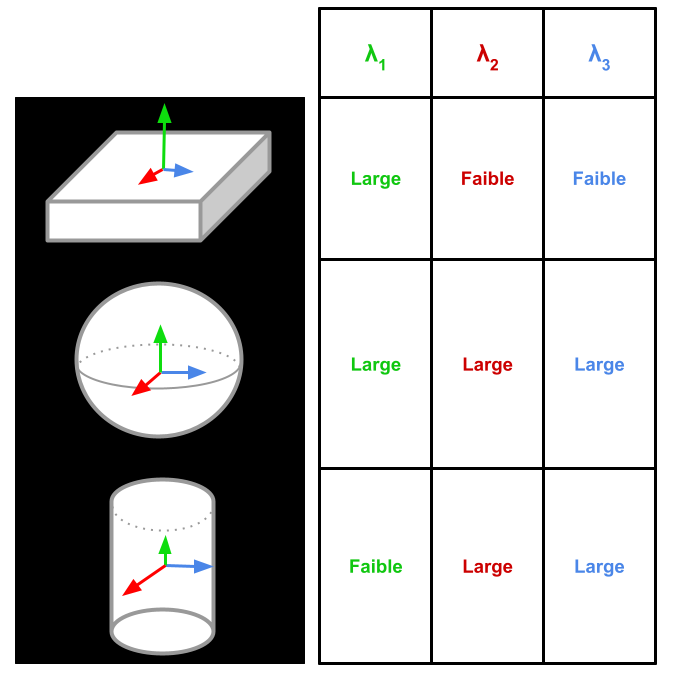
\includegraphics[height=8cm]{Images/table_structures.png}
  \caption{Poids des valeurs propres en fonction de la forme de la géométrie locale. On distingue trois grands types de géométrie : les plateaux, les sphères et les tubes.}
  \label{fig:structures_hessienne}
\end{figure}

\newV{L'équation \ref{eq:tubularity} est la définition idéale d'une structure tubulaire. En pratique, la géométrie d'un réseau vasculaire est complexe. Elle est composée d'un mélange de géométries tubulaires, planaires et sphériques à des degrés divers. Ces structures possèdent parfois des propriétés proches d'élément que l'on ne veut pas rehausser. On peut citer le bruit composé de petites structures sphériques ou encore les bords planaires des organes.}

Plusieurs mesures de tubularité ont donc été proposées dans la littérature afin de différencier au mieux les vaisseaux des autres types de structures. Nous présentons six d'entre elles dans la suite de cette section.
\subsubsubsection{Sato}
Sato \etal \cite{Sato1998_vesselness} sont parmi les premiers à s'appuyer sur la définition de la tubularité \newV{telle qu'exprimée équation \ref{eq:tubularity}.} (N.B. : le tri des valeurs propres est légèrement différent pour Sato. On définit $\lambda^\star_i$ tel que $\lambda^\star_1 \geqslant \lambda^\star_2  \geqslant  \lambda^\star_3$.)
Quand $\lambda^\star_2, \lambda^\star_3 < 0$, le vecteur propre $\mathbf {e^\star_1}$ associé à $\lambda^\star_1$ pointe dans la direction de la plus petite variation d'intensité, qui est aussi la direction du vaisseau.
Dans ce cas, les vecteurs propres $\mathbf {e^\star_2}$ et $\mathbf {e^\star_3}$ forment une base orthogonale à $\mathbf {e^\star_1}$ et correspondent à la coupe transversale du vaisseau.
La taille des axes de la coupe des vaisseaux est proportionnelle à $|\lambda^\star_2|$ et $|\lambda^\star_3|$.

Le filtre de rehaussement de Sato utilise un ratio asymétrique de valeurs propres pour obtenir une réponse forte sur les structures tubulaires, basé sur le signe de $\lambda^\star_1$.
Ce filtre a l'avantage de lisser la réponse et de réduire le bruit. Deux paramètres $\alpha_1$ et $\alpha_2$ contrôlent la force de cette asymétrie :
\begin{equation}
\nonumber
F =
\left\{
\begin{array}{ll}
\lambda^\star_c \exp(-\frac{{\lambda^\star_1}^2}{2(\alpha_1 \lambda^\star_c)^2})  & 
\textrm{Si } \lambda^\star_1 \leqslant 0, \lambda^\star_c \neq 0 \\
\lambda^\star_c \exp(-\frac{{\lambda^\star_1}^2}{2(\alpha_2\lambda^\star_c)^2})  &  
\textrm{Si } \lambda^\star_1 > 0, \lambda^\star_c \neq 0 \\
0 & \textrm{sinon}
\end{array}
\right.
\end{equation}
avec $\lambda^\star_c = \min\{-\lambda^\star_2,-\lambda^\star_3\}$.
\subsubsubsection{Frangi}
Une année plus tard, Frangi \etal \cite{Frangi1998_vesselness} exploitent l'ensemble des valeurs propres afin de proposer un contrôle plus fin de la géométrie des structures rehaussés. Trois mesures sont dérivées des valeurs propres :
\begin{align}
 \nonumber
  R_b & = |\lambda_1| / \sqrt{|\lambda_2\lambda_3|}\\
R_a & = |\lambda_2| / |\lambda_3| \nonumber\\
S & = \sqrt{\lambda^2_1 + \lambda^2_2 + \lambda^2_3} \nonumber
\end{align}
Ces mesures permettent de discriminer les blobs ($R_b$), différencier les plateaux des structures en ligne ($R_a$) et contrôler les structures de faible contraste en étudiant la norme de la hessienne ($S$). Ces trois mesures sont unifiées dans une fonction de rehaussement :   
\begin{align}
  F & = \begin{cases} 
                \big(1-\exp\big(-\frac{R_a^2}{2\alpha^2}\big)\big) \exp\big(-\frac{R_b^2}{2\beta^2}\big)\big(1-\exp(-\frac{S^2}{2C^2}\big)\big), \textrm{~Si~} \lambda_2 \textrm{~et~} \lambda_3 \leqslant 0   \\
                0, \textrm{ sinon} \\
              \end{cases}
\end{align}
Cette fonction est contrôlée par trois paramètres $\alpha$, $\beta$, $C$, qui rendent complexe le paramétrage du filtre. Cette méthode est utilisée dans la plupart des applications de segmentation avec rehaussement.
\subsubsubsection{Meijering}
Meijering et al. \cite{Meijering2004_neurite_vesselness} proposent un filtre pour la détection de neurites dans des images fluoroscopiques. Ils s'intéressent en particulier à rehausser les structures fines d'un ou deux voxels de large grâce à un filtre de détection de structures tubulaires dont l'élongation est maximisée. Cette méthode a ensuite été testée en 3D dans \cite{Obara2012_phase}. Le filtre repose sur une matrice hessienne modifiée $H'(f)$ que nous définissons de la manière suivante :
\begin{equation}
  %\small
    H^{'}(f)=
    \begin{bmatrix}
    \alpha h_{11}+ h_{22} +   h_{33} ~~~~~~~~~ h_{12} ~~~~~~~~~~~~~~~~~~~~~~~~~ h_{13} ~~~~~~~~ \\
    h_{21} ~~~~~~~~~~~~ \alpha h_{22} + h_{11} +  h_{33} ~~~~~~~~~~~~~~ h_{23} \\
    ~~~~~~ h_{31} ~~~~~~~~~~~~~~~~~~ h_{32} ~~~~~~~~~~~~~~ \alpha h_{33} + h_{11} +  h_{22}
    \end{bmatrix}
\end{equation}
avec $h_{ij}$ les dérivées partielles secondes dont les définitions ont été rappelées section \ref{sec:EA:rehaussement:hessienne}.

Le paramètre $\alpha$ est utilisé pour orienter le filtre afin que son élongation soit maximale dans une direction. Meijering avait prouvé pour le cas 2D que la valeur optimale de $\alpha$ était $-1/3$. La preuve de la valeur optimale de $\alpha$ pour le cas 3D, n'a jamais été explicitement documenté. Nous fournissons une preuve en annexe \ref{APP:Proof of Meijering's maximal flatness for 3D case} pour le cas 3D et démontrons que le $\alpha$ optimal est $-2/3$. Les trois valeurs propres de $H'(f)$ sont exprimées en fonction de celles de $H(f)$ comme :
\begin{equation}
  \begin{aligned}
    \nonumber \lambda_1' = \alpha\lambda_1 + \lambda_2 + \lambda_3 \\
    \nonumber \lambda_2' = \lambda_1 + \alpha\lambda_2 + \lambda_3 \\
    \nonumber \lambda_3' = \lambda_1 + \lambda_2 + \alpha\lambda_3
  \end{aligned}
\end{equation}
La mesure de tubularité est alors :
\begin{equation}
\nonumber 
  F =
  \left\{
  \begin{array}{lr}
    \lambda_{\max} / \lambda_{\min}   &  \lambda_{\max} < 0\\
      0 &  \lambda_{\max} \geqslant 0
  \end{array}
  \right.
\end{equation}
où $\lambda_{max} = \max\{\lambda_{1}^{'},\lambda_{2}^{'},\lambda_{3}^{'}\}$ est calculé pour chaque voxel, et $\lambda_{min}$ est la valeur propre minimale parmi \newV{l'ensemble des valeurs propres calculées pour tous les pixels de l'image.}
\subsubsubsection{OOF}
\newV{Pour le flux orienté, Law et al. \cite{Law2008_OOF} proposent d'utiliser différentes combinaisons de valeurs propres. Dans le cas de leurs expériences sur des données réelles, ils utilisent la moyenne géométrique des valeurs propres de la coupe transversale des vaisseaux :}
\begin{equation}
\nonumber
    F =
    \left\{
    \begin{array}{lr}
    
    \sqrt{|\lambda_2 \cdot \lambda_3|}   & \lambda_2, \lambda_3 < 0 \\
    0     & \textrm{sinon}
    \end{array}
    \right.
\end{equation}
\subsubsubsection{Jerman}
Jerman et al. ont proposé une fonction de rehaussement dont l'objectif est de renforcer le signal aux bifurcations tout en proposant un filtre plus simple à paramétrer que le filtre de Frangi. Le rehaussement proposé repose sur la mesure \textit{volume aspect ratio}, utilisée pour détecter des tenseurs presque sphériques. La fonction est définie par :
\begin{equation}
\nonumber
  F =
\left\{
  \begin{array}{lll}
    0 & \lambda_2 \leqslant & \textrm{~ou~} \lambda_\rho \leqslant 0 \\
    1 & \lambda_2 \geqslant & \lambda_\rho / 2 > 0 \\
    \lambda_{2}^2(\lambda_\rho -\lambda_2)\big(\frac{3}{\lambda_2+\lambda_\rho}\big)^3 & \textrm{sinon} &
  \end{array}
  \right. 
\end{equation}
$\lambda_\rho$ est la version régularisée de la valeur propre $\lambda_3$, défini pour réduire la sensibilité du filtre aux régions peu contrastées :
\begin{equation}
\nonumber
  \lambda_\rho =
  \left\{
  \begin{array}{ll}
     \lambda_3  & \lambda_3 > \tau \max_{x} \lambda_3(x) \\
    \tau \max_{x} \lambda_3(x) & 0 < \lambda_3 \leqslant \tau \max_{x} \lambda_3(x) \\
    0  & \textrm{sinon}
  \end{array}
\right.
\end{equation}
où $\tau \in [0,1]$. Cette paramétrisation produit une réponse du filtre plus homogène, même pour des vaisseaux avec des profils non homogènes.
\subsubsubsection{Zhang}
Zhang et al. \cite{Zhang2018_liver_fuzzy_connectedness} proposent d'améliorer le rehaussement de Jerman dans le contexte de la segmentation de vaisseaux hépatiques, et plus particulièrement sur le foie masqué. Pour résoudre ce problème de réponses fortes sur les bords du foie, les auteurs proposent une classification à base de K-moyennes pour estimer les intensités moyennes des vaisseaux. Ils utilisent ensuite ces intensités moyennes pour paramétrer une fonction sigmoïde pour filtrer les autres tissus. De plus, ils modifient légèrement le rehaussement de Jerman $F$ en ajoutant un terme multiplicatif $1-e^{ \frac{-R^2_s}{2 \gamma}}$ avec $R_s = \sqrt{\lambda^2_1 + \lambda^2_2 + \lambda^2_2}$ et $\gamma= \frac{\lambda_p}{3}$.
\subsection{Filtres basés morphologie mathématique}
\subsubsection{Espace d'échelles granulométrique}
\label{sec:EA:rehaussement:echelle:granulometrie}
La granulométrie est l'étude des tailles des particules d'un échantillon. En chimie, on utilise par exemple la technique du tamisage. Elle permet, grâce à un tamis et une grille dont on contrôle la taille du maillage, de ne conserver que des particules dont la taille est trop grosse pour passer à travers le tamis. Un principe similaire est applicable en morphologie mathématique sur les images binaires et par extension en niveaux de gris. \newV{En morphologie mathématique, la forme et la taille du maillage du tami sont exprimés par l'élément structurant.}
\subsubsubsection{Érosion et dilatation}
Deux opérations élémentaires, la dilatation et l'érosion, permettent de définir les opérations nécessaires pour construire un espace d'échelles morphologique. Les définitions qui vont suivre sont des opérations binaires relatives à des objets blancs sur fond noir.
\paragraph{Définitions}
% definition de Digital image processing, Gonzalez second edition, Mophology - p518
Soit deux ensembles $A$ et $B$ définis dans $\mathbb{Z}^3$ tels que $a=(a_1,a_2,a_3)  \in A$ et $b=(b_1,b_2,b_3) \in B$.

Soit une image binaire $I$ définie sur $Z^3$ composé d'un ensemble blanc $A$ sur fond noir. On appelle élément structurant un ensemble $B_p$ avec $p$ son ancre. $p$ peut être défini en dehors de B, mais on préfère en général définir l'ancre comme étant le centre de l'élément structurant afin d'éviter la translation des structures de l'image.
\paragraph{Dilatation}
La dilatation d'un ensemble $A$ par l'élément structurant $B_p$ s'exprime par :
\begin{equation}
A \oplus B_p = \bigcup_{p \in A}B_{p} \
\end{equation}
La dilatation de A par $B_p$ est l'ensemble de tous les déplacements de $B_p$ tels que $p$ soit inclus dans A. Cette opération permet de faire grossir une structure en fonction de la forme de $B_p$ (Fig. \ref{fig:morpho_dilation}).
\begin{figure}[!ht]
  \centering
  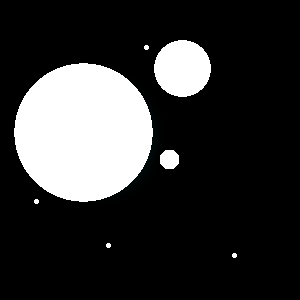
\includegraphics[height=3cm]{Images/morpho_init.png}
  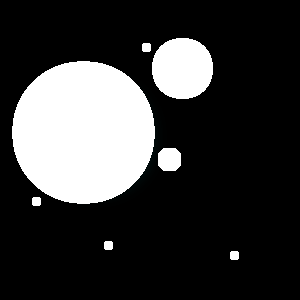
\includegraphics[height=3cm]{Images/morpho_dilate_k5.png}
  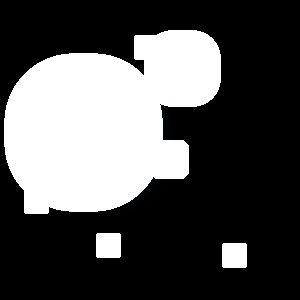
\includegraphics[height=3cm]{Images/morpho_dilate_k21.png}
  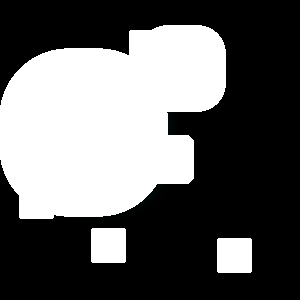
\includegraphics[height=3cm]{Images/morpho_dilate_k31.png}
  \caption{Exemple de dilatation par un élément structurant rectangulaire. La dilatation fait grossir les structures selon la forme de l'élément structurant.}
  \label{fig:morpho_dilation}
\end{figure}

\paragraph{Érosion}
L'opération complémentaire à la dilatation est l'érosion (Fig. \ref{fig:morpho_erosion}) :
\begin{equation}
  A \ominus B_p = \{p, B_p \subseteq A\}
\end{equation}
L'érosion de $A$ par $B_p$ est l'ensemble de tous les points $p$ tel que $B_p$ est inclus dans $A$. 
\begin{figure}[!ht]
  \centering
  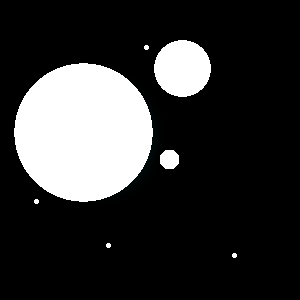
\includegraphics[height=3cm]{Images/morpho_init.png}
  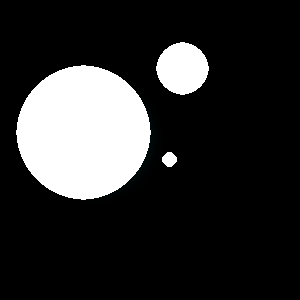
\includegraphics[height=3cm]{Images/morpho_erode_k5.png}
  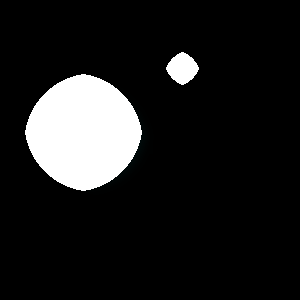
\includegraphics[height=3cm]{Images/morpho_erode_k21.png}
  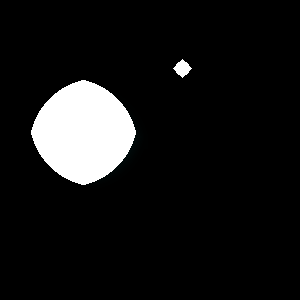
\includegraphics[height=3cm]{Images/morpho_erode_k31.png}
  \caption{Exemple d'érosion avec un élément structurant rectangulaire. L'érosion peut faire disparaître des petites structures et érode les structures en fonction de la géométrie de l'élément structurant.}
  \label{fig:morpho_erosion}
\end{figure}
\subsubsubsection{Fermeture et ouverture}
À partir des opérations d'érosion et de dilatation, on peut définir des opérations composites : l'ouverture et la fermeture.
\paragraph{Fermeture}
La fermeture est définie comme la dilatation de $A$ par $B_p$ suivi de l'érosion du résultat par $B_p$.
\begin{equation}
 A \bullet B_p = (A \oplus B_p) \ominus B_p
\end{equation}  
Cet opérateur est utilisé pour boucher les trous et les concavités dont la surface est inférieure à la surface de l'élément structurant (Fig. \ref{fig:morpho_femerture}). L'érosion qui suit la dilatation permet d'assurer que la taille reste stable.
\begin{figure}[!ht]
  \centering
  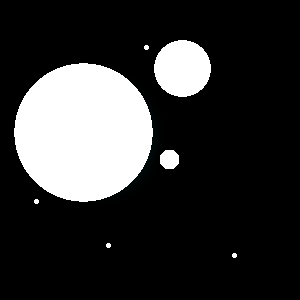
\includegraphics[height=3cm]{Images/morpho_init.png}
  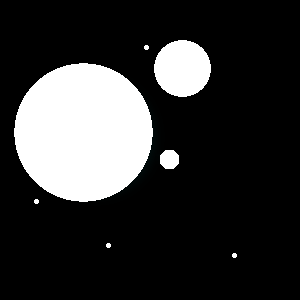
\includegraphics[height=3cm]{Images/morpho_close_k5.png}
  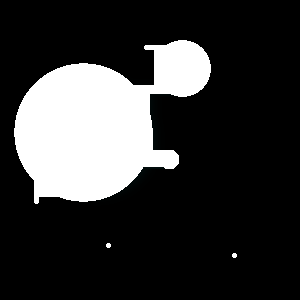
\includegraphics[height=3cm]{Images/morpho_close_k21.png}
  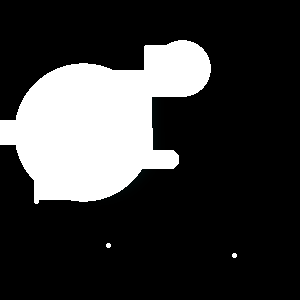
\includegraphics[height=3cm]{Images/morpho_close_k31.png}
  \caption{Exemple de fermeture par un élément structurant rectangulaire. La fermeture reconnecte des éléments adjacents en fonction de la géométrie de l'élément structurant.}
  \label{fig:morpho_femerture}
\end{figure}

\paragraph{Ouverture}
L'ouverture est définie comme l'érosion de $A$ par $B_p$ suivie de la dilatation du résultat par $B_p$.
\begin{equation}
 A \circ B_p = (A \ominus B_p) \oplus B_p
\end{equation}
\begin{figure}[!ht]
  \centering
  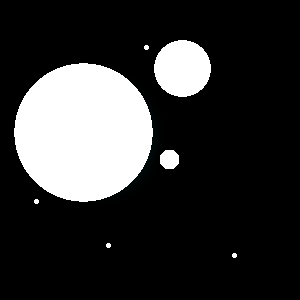
\includegraphics[height=3cm]{Images/morpho_init.png}
  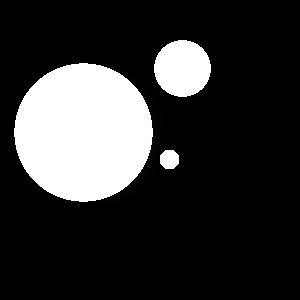
\includegraphics[height=3cm]{Images/morpho_open_k5.png}
  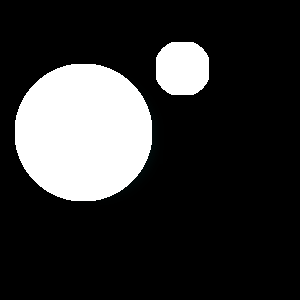
\includegraphics[height=3cm]{Images/morpho_open_k21.png}
  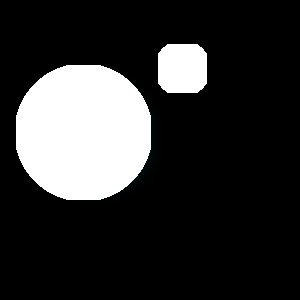
\includegraphics[height=3cm]{Images/morpho_open_k31.png}
  \caption{Exemple d'ouverture. L'augmentation de la taille de l'élément structurant fait disparaitre les structures dont la surface ne peut inclure l'élément structurant. L'espace d'échelles formé par une ouverture se comporte comme un espace d'échelles gaussien en conservant toutes les structures de tailles supérieure à la taille de l'élément structurant. }
  \label{fig:morpho_ouverture}
\end{figure}

L'opérateur d'érosion est utilisé pour supprimer les structures et convexités de taille inférieure à la surface de l'élément structurant (Fig. \ref{fig:morpho_ouverture}). La dilatation qui suit l'érosion permet d'assurer que la taille des éléments reste stable.
\newV{En utilisant l'ouverture, on peut définir un espace d'échelles qui se comporte comme un espace d'échelles gaussien. C'est-à-dire que plus la taille de l'élément structurant augmente et plus on élimine des structures de grande taille. Cet espace ne souffre pas d'une fusion parasite des structures adjacentes.}
\subsubsubsection{Morphologie en niveaux de gris}
Les opérations que nous avons définies jusqu'à maintenant sont applicables pour les images binaires. Pour des images de niveaux de gris les filtres \emph{min} et \emph{max} sont analogues à l'érosion et la dilatation binaire.

Ainsi la dilatation en niveaux de gris est définie pour chaque voxel à la position $p$ par le maximum de la valeur des voxels $p_x$ de l'image $I$  compris dans la zone de l'élément structurant $B_p$ :
\begin{equation}
I \oplus_{ng} B_p = \max_{p_x \in B_p} I(p_x) \
\end{equation}
L'érosion est définie pour chaque voxel à la position $p$ par le minimum de la valeur des voxels $p_x$ de l'image $I$ compris dans la zone de l'élément structurant $B_p$ :
\begin{equation}
  I \ominus_{ng} B_p = \min_{p_x \in B_p} I(p_x) \
\end{equation}
Les opérations d'ouvertures et de fermetures sont définies de manière analogue aux ouvertures et fermetures binaires. La fermeture est définie par :
\begin{equation}
I \bullet B_p = (I \oplus_{ng} B_p) \ominus_{ng} B_p
\end{equation}
L'ouverture est définie par : 
\begin{equation}
  I \circ B_p = (I \ominus B_p) \oplus B_p
 \end{equation}
 Ces opérations possèdent les mêmes propriétés que leur contrepartie binaire appliquée à l'intensité des voxels (Fig. \ref{fig:greyscale_morpho}). La taille de l'élément structurant joue le même effet de sélection de l'échelle des structures de l'image que dans le cas binaire. 
 \begin{figure}
  %  trim={<left> <lower> <right> <upper>}
  \begin{subfigure}[t]{0.30\textwidth}
    \centering
    \adjincludegraphics[width=\textwidth,trim={{0.1\width} {0.05\height} {0\width} {0.1\height}},clip]{Images/ng_1.png}
    \caption{original}
  \end{subfigure}
  \begin{subfigure}[t]{0.30\textwidth}
    \centering
    \adjincludegraphics[width=\textwidth,trim={{0.1\width} {0.05\height} {0\width} {0.1\height}},clip]{Images/ng_dilate.png}
    \caption{dilatation}
  \end{subfigure}
  \begin{subfigure}[t]{0.30\textwidth}
    \centering
    \adjincludegraphics[width=\textwidth,trim={{0.1\width} {0.05\height} {0\width} {0.1\height}},clip]{Images/ng_erode.png} 
    \caption{érosion}
  \end{subfigure}
  \centering
  \begin{subfigure}[t]{0.30\textwidth}
    \centering
    \adjincludegraphics[width=\textwidth,trim={{0.1\width} {0.05\height} {0\width} {0.1\height}},clip]{Images/ng_close.png}
    \caption{fermeture}
  \end{subfigure}
  \begin{subfigure}[t]{0.30\textwidth}
    \centering
    \adjincludegraphics[width=\textwidth,trim={{0.1\width} {0.05\height} {0\width} {0.1\height}},clip]{Images/ng_open.png}  
    \caption{ouverture}
  \end{subfigure}  
  \caption{Opérateurs morphologiques appliqués aux images en niveaux de gris. L'élément structurant utilisé est un carré de $3\times3$.}
  \label{fig:greyscale_morpho}
\end{figure}

\subsubsection{Descripteur de géométrie par éléments structurants}
\label{sec:EA:rehaussement:morpho}
\newV{Pour le rehaussement des vaisseaux, on utilise une composition d'ouvertures dont les éléments structurants sont des boules et des cylindres. Les cylindres permettent de couvrir les parties curvilignes des vaisseaux, tandis que les boules couvrent les jonctions.} Sazak et al. proposent un schéma de ce type en 2D \cite{Sazak2019_bowler_hat_2D} et en 3D \cite{Sazak2018_bowler_hat_3D} et comparent son efficacité relativement au rehaussement à base de tenseurs de phase et hessien. Cette méthode bien que simple à mettre en pratique, nécessite plusieurs itérations avec des rotations des éléments structurants afin de capturer toutes les orientations des structures tubulaires. Elle peut ainsi rapidement devenir coûteuse en 3D.
\begin{figure}[!ht]
\centering
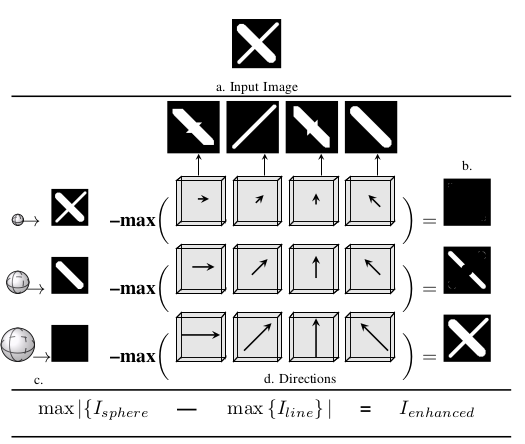
\includegraphics[height=9cm]{Images/bowlerHat_3D.png}
\caption{\textit{Bowler hat transform} proposée par Sazak et al. \cite{Sazak2018_bowler_hat_3D} La combinaison d'éléments sphériques et linéaires permet de capturer les structures curvilinéaires. }
\label{fig:sazak_bowler_hat}
\end{figure}

L'un des défauts de la méthode que nous venons d'exposer est le caractère fixe des éléments structurants qui ne permettent pas toujours de capturer les variations de formes des vaisseaux. Hejimans et al. \cite{Heijmans2005_path_opening} proposent une famille d'éléments structurants variables dont la forme est définie par une grille d'adjacences. Des améliorations successives de cet algorithme ont été proposés : Cokelaer et al. \cite{Cokelaer2012_efficient_path_opening} proposent une version robuste au bruit en autorisant des discontinuités dans l'élément structurant, Van de Gronde et al. \cite{Gronde2015_fast_path_opening} proposent une implémentation efficace de l'algorithme en $O( N log ( L ))$ avec $N$ le nombre de pixels de l'image et $L$ la taille du chemin. Enfin Merveille et al. \cite{Merveille2018_curvilinear} itèrent sur la méthode en proposant un classement de l'orientation des chemins afin de segmenter les vaisseaux dans des images 2D et 3D (Sec. \ref{sec:sub_rorpo}). 
\subsubsubsection{RORPO}
\label{sec:sub_rorpo}
RORPO \cite{Merveille2018_curvilinear} est construit sur un espace d'échelles granulométrique défini par des ouvertures de chemins. Pour capturer les structures curvilinéaires, les éléments structurants sont définis comme des chemins sur une grille d'adjacence qui fournit un cadre flexible sur la géométrie des éléments à détecter (Fig. \ref{fig:rorpo_adjacency}). 
\begin{figure}[!ht]
\centering
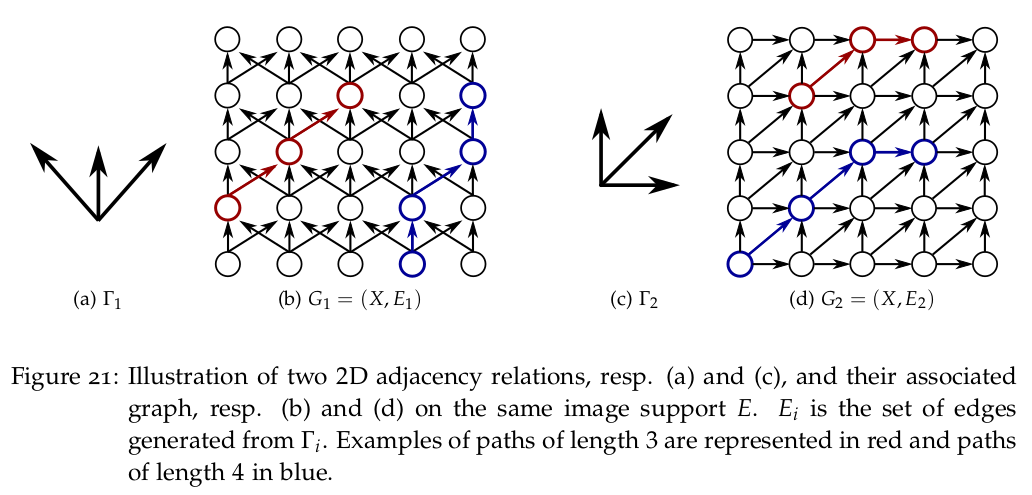
\includegraphics[height=4cm]{Images/rorpo_path.png}
\caption{Illustration de relations d'adjacence permettant de définir les éléments structurants de RORPO. Cette relation est définie par rapport à un graphe $G_i$ défini par un ensemble de nœuds $E_i$ et d'arêtes $E_i$. L'ensemble des arêtes est défini selon un ensemble d'orientations spécifiques $\Gamma_i$. Les éléments structurants définis pour ces orientations détectent l'ensemble des structures de même nature orientées de la même manière.}
\label{fig:rorpo_adjacency}
\end{figure}

Les ouvertures sont calculées avec des éléments structurants définis dans 7 orientations principales de l'espace 3D de manière à capturer les objets de différentes formes tels que les blobs, les structures linéaires et les plateaux. Une étape finale consiste à classifier les différentes formes en triant les orientations des éléments structurants. En effet, pour des objets tubulaires, tous les éléments structurants sont orientés dans la même direction. RORPO est complétement lié à son espace d'échelles (Sec. \ref{sec:EA:rehaussement:echelle:granulometrie}), contrairement aux mesures de tubularité basées sur des valeurs propres qui peuvent s'adapter à plusieurs espaces (gaussien, flux, phase).
\subsection{Multi-échelle}
  \label{sec:EA:rehaussement:echelle:multiScale}
  \newV{Jusqu'à maintenant, nous avons présenté la manière de sélectionner une seule échelle en fonction de l'espace d'échelles choisi (gaussien, de flux ou granulométrique).} Pour capturer l'ensemble des variations de tailles du réseau vasculaire, il suffit d'appliquer les filtres de tubularité sur un ensemble d'échelles, une à une. Les résultats de ces traitements sont rarement exploités séparément. À la place, ils sont fusionnés dans une seule et même réponse grâce à un opérateur $\max$. Cet opérateur permet de récupérer pour un pixel donné la réponse maximale à travers l'ensemble des échelles.

  De manière explicite, le résultat du filtre de rehaussement $R_{multi echelle}$ est défini comme le maximum des rehaussements $R_{p}$ appliqués à l'image I à l'échelle $p$ :
  \begin{equation}
    R(I)_{multi \acute echelle} = \max_{p}R_{p}(I) 
  \end{equation}
  \newV{Le paramètre $p$ dépend de l'espace d'échelles utilisé et correspond soit à $\sigma$ pour l'espace gaussien, le rayon de la sphère de l'espace de flux et la taille de l'élément structurant pour l'espace granulométrique.}
  
  Cet opérateur peut provoquer un recouvrement des structures rehaussées par une structure adjacente ayant une réponse plus forte à un filtre. À notre connaissance, aucune publication ne propose de pondérer ou de hiérarchiser la réponse en fonction de la taille du noyau (gaussienne, élément structurant, sphère, etc.) de l'espace d'échelles.

  Le choix de l'intervalle d'un espace multi-échelles est contrôlé par une borne inférieure, une borne supérieure et un nombre d'échelles dans cet intervalle. De manière naïve, on pourrait choisir d'espacer les échelles linéairement sur l'intervalle. Pour les vaisseaux, plus ceux-ci sont fins et plus leur nombre augmente. Il est donc nécessaire de consacrer un plus grand nombre de petites échelles  et un nombre plus réduit de grandes échelles pour capturer efficacement l'ensemble des réseaux vasculaires. On préfère donc utiliser un espace d'échelles logarithmique à un espace d'échelles linéaire (Fig. \ref{fig:scale_space}).
  \begin{figure}[!ht]
    \centering
    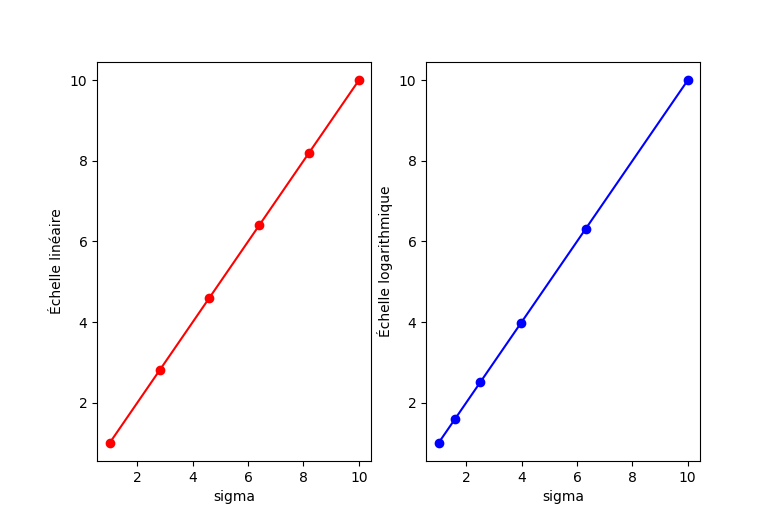
\includegraphics[height=6cm]{Images/scale_space.png}
    \caption{Représentation de l'espace gaussien dans lequel $\sigma$ est le paramètre d'échelle. Espace d'échelles linéaire vs. espace d'échelles logarithmique : $\sigma_{inf}=1, \sigma_{sup}=10, \textrm{nombre d'échelles}=6$. Avec l'échelle logarithmique, les variations des petits vaisseaux sont mieux capturées.}
    \label{fig:scale_space}
  \end{figure}

\subsection{Amélioration des filtres par diffusion}
\label{sec:EA:rehaussement:diffusion}
On ne peut aborder les filtres de rehaussement de vaisseaux sans aborder les cadres de diffusions. Leur objectif est d'améliorer le signal des vaisseaux en homogénéisant leur intensité et en renforçant leurs bords. Pour cela, les filtres de diffusion proposent un schéma de lissage itératif qui prend en compte la géométrie des structures à lisser.

\newV{HDCS \cite{Mendrik2009_HDCS} (Hybrid diffusion with continuous switch), propose un lissage hybride qui permet de choisir un type de lissage spécifique en fonction du voisinage du voxel traité. Un lissage isotrope est appliqué dans les régions d'intensités quasi constantes et un lissage anisotrope est utilisé le long des bordures des structures. La transition entre les types de lissage en fonction des régions est assurée par une combinaison linéaire des deux filtres pondérés par une mesure de la géométrie locale.}

VED \cite{Manniesing2006_VED} (Vessel enhancement diffusion) propose un lissage basé sur les méthodes de rehaussement hessien. Ce cadre permet ainsi d'homogénéiser la réponse de n'importe quel filtre de rehaussement hessien en lissant selon le sens du rehaussement.
\begin{figure}[!ht]
  \centering
  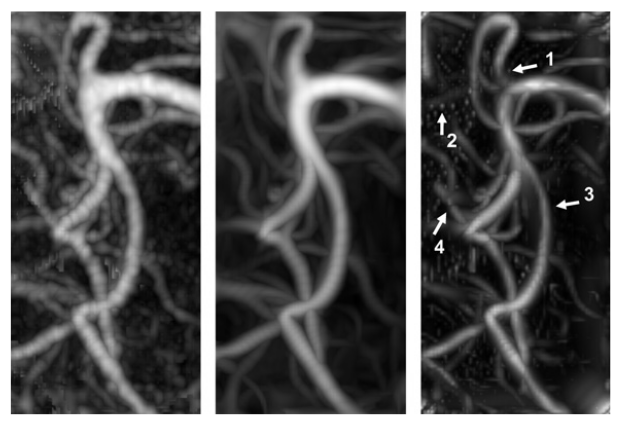
\includegraphics[height=8cm]{Images/VED.png}
  \caption{Comparaison de l'image originale (gauche), VED+Frangi (centre) et Frangi (droite). Le rehaussement est lissé et l'homogénéité générale des vaisseaux est renforcée. Les flèches montrent les différences de comportement remarquables.}
  \label{fig:custom_fig}
\end{figure}

Ces méthodes itératives sont coûteuses en temps de calcul et nécessitent une paramétrisation supplémentaire pour contrôler la force du lissage ainsi que le nombre d'itérations nécessaire.
\section{Bilan et orientation des travaux}
\label{sec:EA:bilan}
Les constatations pour l'état de l'art du rehaussement de vaisseaux sont sensiblement les mêmes que celles dressées pour le bilan de l'état de l'art sur la segmentation (Sec. \ref{sec:problems_segmenation}). Les articles originaux testent souvent leurs méthodes sur des structures synthétiques simples ou des exemples variés. Elles sont toujours comparées à deux à quatre autres méthodes. Lorsqu'ils sont utilisées sur des données réelles, les filtres de rehaussement sont largement appliqués avec les paramètres recommandés par l'auteur, sans adaptation à une application particulière.

Quelques travaux portent sur la comparaison des filtres de rehaussement. Luu et al. \cite{Luu2015_liver_vesselness_comparison} proposent une comparaison de trois filtres de rehaussement et trois filtres de diffusion pour la tomodensitométrie du foie. Phellan et al. \cite{Phellan2017_Brain_vesselness_comparison} proposent une comparaison de six filtres de rehaussement et trois filtres de diffusion sur des images d'IRM du cerveau et un jeu de données synthétiques.

Cependant, ces travaux ne nous permettent pas de répondre à plusieurs questions~:
\begin{itemize}
\item quel filtre utiliser pour l'IRM du foie ?
\item quel est l'impact de la paramétrisation sur la réponse des filtres ?
\item La taille des vaisseaux a t'elle un impact sur la qualité du rehaussement ?
\item quel est l'impact des filtres de rehaussement indépendamment de la segmentation ?
\end{itemize}
Dans le chapitre suivant, nous élaborons la construction d'un banc de tests pour étudier ces problématiques. Celui-ci nous permettra ensuite d'effectuer une analyse poussée des filtres de rehaussement des vaisseaux sanguins dans les chapitres suivants.








